\section{Formalism}
\subsection*{Sol. 1}
\begin{enumerate}
    \item Given two square integrable functions $f$ and $g:$
    \begin{align*}
        \int (f+g)^*(f+g)=&
        \int f^*f + \int g^*g 
        +\int f^*g + \int g^*f
    \end{align*}
    By eq3.7
    $$
    \left|\int f^*g\right|
    \leq \sqrt{\int f^*f\cdot \int g^*g} < \infty,
    $$
    therefore $ \int (f+g)^*(f+g)<\infty.$
    The set of normalized functions is obviously not a vector space.
    \item 
    \begin{itemize}
        \item 
        $$
        \langle
        f+g|h
        \rangle
        =
        \int(f+g)^*h
        =\int f^*h + \int g^*h
        =\langle
        f|h
        \rangle
        +\langle
        g|h
        \rangle
        $$
        \item 
        $$
        \langle f|cg\rangle
        =
        \int f^*(cg)
        =
        c\int f^*g
        =c\langle f|g\rangle
        $$
        \item 
        $$
        \overline{
        \langle f|g\rangle
        }
        =
        \overline{\int f^*g}
        =
        \int g^*f
        =\langle g|f\rangle
        $$
        \item 
        If $f\neq 0$
        $$
        \langle f|f\rangle
        =\int |f|^2 >0
        $$ by eq3.9.
    \end{itemize}
\end{enumerate}
\subsection*{Sol. 2}
\begin{enumerate}
    \item 
    $$
    \int_0^1 x^{2\nu}dx = \frac{1}{2\nu+1},
    $$
    if $2\nu>-1,$  and 
    $$
    \int_0^1 x^{2\nu}dx > \infty,
    $$
    if $2\nu<-1.$
    \item $x^{1/2}$ is in this Hilbert space. $x^{3/2}$ is in this Hilbert space. $\frac{1}{2}x^{-1/2}$ is not.

\end{enumerate}

\subsection*{Sol. 3}
For any $f$ and $g,$
\begin{align*}
    \langle f+g|\hat{Q}(f+g)\rangle
    =\langle f|\hat{Q}f\rangle+
    \langle f|\hat{Q}g\rangle+
    \langle g|\hat{Q}f\rangle+
    \langle g|\hat{Q}g\rangle
\end{align*}
\begin{align*}
    \langle \hat{Q}(f+g)|f+g\rangle
    =\langle \hat{Q}f|f\rangle+
    \langle \hat{Q}f|g\rangle+
    \langle \hat{Q}g|f\rangle+
    \langle \hat{Q}g|g\rangle
\end{align*}
We have 
$$
\langle f|\hat{Q}g\rangle+
\langle g|\hat{Q}f\rangle
=\langle \hat{Q}f|g\rangle+
\langle \hat{Q}g|f\rangle.
$$

\begin{align*}
    \langle f+ig|\hat{Q}(f+ig)\rangle
    =\langle f|\hat{Q}f\rangle+
    i\langle f|\hat{Q}g\rangle
    -i\langle g|\hat{Q}f\rangle+
    \langle g|\hat{Q}g\rangle
\end{align*}
\begin{align*}
    \langle \hat{Q}(f+ig)|f+ig\rangle
    =\langle \hat{Q}f|f\rangle+
    i\langle \hat{Q}f|g\rangle
    -i\langle \hat{Q}g|f\rangle+
    \langle \hat{Q}g|g\rangle
\end{align*}
We have 
$$
\langle f|\hat{Q}g\rangle
-\langle g|\hat{Q}f\rangle
=\langle \hat{Q}f|g\rangle
-\langle \hat{Q}g|f\rangle.
$$

Summing these two conditions, we obtain
$$
\langle f|\hat{Q}g\rangle=\langle \hat{Q}f|g\rangle.
$$

\subsection*{Sol. 4}
\begin{enumerate}
    \item 
    \begin{align*}
    \langle f|(\hat{Q}+\hat{R})f\rangle
    =&
    \langle f|\hat{Q}f\rangle+
    \langle f|\hat{R}f\rangle\\
    =&
    \langle \hat{Q}f|f\rangle+
    \langle \hat{R}f|f\rangle\\
    =&
    \langle \hat{Q}f|f\rangle+
    \langle \hat{R}f|f\rangle\\
    =&\langle (\hat{Q}+\hat{R})f|f\rangle
    \end{align*}
    \item 
    $$
    \langle \alpha\hat{Q}f|f\rangle
    =
    \alpha
    \langle \hat{Q}f|f\rangle
    $$
    $$
    \langle f|\alpha\hat{Q}f\rangle=
    \alpha^*
    \langle f|\hat{Q}f\rangle
    $$
    $\alpha$ has to be real.
    \item 
    \begin{align*}
    \langle f|\hat{Q}\hat{R}f\rangle
    =&
    \langle \hat{Q}f|\hat{R}f\rangle\\
    =&\langle \hat{R}\hat{Q}f|f\rangle
    \end{align*}
    When these two hermitian operators commute, their product is hermitian.
    \item 
    \begin{align*}
        \langle f|\hat{x}f\rangle
        =& 
        \int f^* xf\\
        =& 
        \int (xf)^* f\\
        =&\langle \hat{x}f|f\rangle
    \end{align*}
    \begin{align*}
        \langle f|\hat{H}f\rangle
        =& 
        \int f^* \left(-\frac{\hbar^2}{2m}\frac{d^2}{dx^2}+V\right)f\\
        =& 
        -\frac{\hbar^2}{2m}\int f^* f'' + \int Vf^*f
    \end{align*}
    Note that using integration by parts
    $$
    \int f^* f''= -\int f'^*f' = \int f''^*fnx,
    $$
    so 
    \begin{align*}
        \langle f|\hat{H}f\rangle=&
        -\frac{\hbar^2}{2m}\int f''^* f + \int Vf^*f\\
        =&\langle \hat{H}f|f\rangle.
    \end{align*}
    
    
    
\end{enumerate}

\subsection*{Sol. 5}
\begin{enumerate}
    \item 
    $$
    \langle
    f|xg
    \rangle=\int f^*xg
    =\int (xf)^*g
    =
    \langle
    xf|g
    \rangle
    $$

    $$
    \langle
    f|ig
    \rangle=\int f^*ig
    =\int (-if)^*g
    =
    \langle
    -if|g
    \rangle
    $$

    $$
    \langle
    f|\frac{d}{dx}g
    \rangle=\int f^*g'
    =\int -f'^*g
    =
    \langle
    -\frac{d}{dx}f|g
    \rangle
    $$
    \item 
    \begin{align*}
        \langle f|\hat{Q}\hat{R}g\rangle
        =& 
        \langle \hat{Q}^\dagger f|\hat{R}g\rangle\\
        =& 
        \langle \hat{R}^\dagger\hat{Q}^\dagger f|g\rangle
    \end{align*}

    \begin{align*}
        \langle f|(\hat{Q}+\hat{R})g\rangle
        =& 
        \langle f|\hat{Q}g\rangle
        +
        \langle f|\hat{R}g\rangle\\
        =& 
        \langle \hat{Q}^\dagger f|g\rangle + 
        \langle \hat{R}^\dagger f|g\rangle\\
        =&
        \langle (\hat{Q}+\hat{R})^\dagger f|g\rangle
    \end{align*}

    \begin{align*}
        \langle f|(c\hat{Q})g\rangle
        =& 
        c\langle f|\hat{Q}g\rangle\\
        =& 
        c\langle \hat{Q}^\dagger f|g\rangle\\
        =&
        \langle c^*\hat{Q}^\dagger f|g\rangle
    \end{align*}
    \item 
    $$
    \hat{a}_+^\dagger = \frac{1}{\sqrt{2\hbar m\omega}}
    (-i\hat{p}+m\omega x)^\dagger 
    =
     \frac{1}{\sqrt{2\hbar m\omega}}
     (i\hat{p}+m\omega x)=\hat{a}_-
    $$
\end{enumerate}

\subsection*{Sol. 6}
\begin{align*}
    \langle f|\frac{d^2}{d\phi^2}g
    \rangle
    =& 
    \int_0^{2\pi}
    f^*g''\\
    =& - \int_0^{2\pi}f'^*g'\\
    =&\int_0^{2\pi}f''^*g\\
    =&\langle \frac{d^2}{d\phi^2}f|g\rangle
\end{align*}
$
\hat{Q}=\frac{d^2}{d\phi^2}
$
is hermitian.

The eigenvalue equation
$$
f''=qf
$$
has the general solution
$$
f(\phi)
=Ae^{\sqrt{q}\phi}+Be^{-\sqrt{q}\phi}
$$

The condition $f(\phi+2\pi)=f(\phi)$ requires that $e^{\sqrt{q}2\pi}=1.$ Restricting the possible values of $q=-n^2,$ where $n=0,1,2,\dots$ The spectrum is degenerate except for $q=0.$

\subsection*{Sol. 7}
\begin{enumerate}
    \item 
    $$
    \hat{Q}(af+bg)=a\hat{Q}f + b\hat{Q}g=q(af+bg)
    $$
    \item 
    $$
    \frac{d^2}{dx^2}e^x = e^x
    $$
    $$
    \frac{d^2}{dx^2}e^{-x} = e^{-x}
    $$

    Applying the Gram Schmidt process,
    \begin{align*}
        g - \frac{\langle g|f\rangle}{\langle f|f\rangle}f
        =&e^{-x} - \frac{\int_{-1}^11dx}{\int_{-1}^1e^{2x}dx}e^x\\
        =&e^{-x}-\frac{4}{e^{2}-e^{-2}}e^x.
    \end{align*}
    This function is orthogonal to $e^x.$
    
\end{enumerate}

\subsection*{Sol. 8}
\begin{enumerate}
    \item The eigenvalues are $0,\pm1,\pm2,\dots,$ obviously real.
    Given two eigenvalues $q_1\neq q_2$
    $$
    \int (e^{-iq_1\phi})^*e^{-iq_2\phi}d\phi
    =\frac{1}{i(q_1-q_2)}
    e^{i(q_1-q_2)\phi}\bigg|^{2\pi}_0 = 0.
    $$
    \item 
    For prob3.6, the eigenvalues are real.
    Given two eigenvalues $q_1=-n_1^2\neq q_2=-n_2^2$
    \begin{align*}
        &\int (A_1e^{\sqrt{q_1}\phi}+B_1e^{-\sqrt{q_1}\phi})^*
    (A_2e^{\sqrt{q_2}\phi}+B_2e^{-\sqrt{q_2}\phi})d\phi\\
    =&
    \int (A_1^*e^{-in_1\phi}+B_1^*e^{in_1\phi})
    (A_2e^{in_2\phi}+B_2e^{-in_2\phi})d\phi\\
    =& A_1^*A_2 \frac{1}{i(-n_1+n_2)}e^{i(-n_1+n_2)}
    \bigg|^{2\pi}_0
    +
    A_1^*B_2 \frac{1}{i(-n_1-n_2)}e^{i(-n_1-n_2)}
    \bigg|^{2\pi}_0\\
    &+
    B_1^*A_2 \frac{1}{i(n_1+n_2)}e^{i(n_1+n_2)}
    \bigg|^{2\pi}_0+
    B_1^*B_2 \frac{1}{i(n_1-n_2)}e^{i(n_1-n_2)}
    \bigg|^{2\pi}_0
     \\
    =& 0.
    \end{align*}
    
\end{enumerate}


\subsection*{Sol. 9}
\begin{enumerate}
    \item The infinite potential well has only a discrete spectrum.
    \item The positive delta function potential has only a continuous spectrum. 
    \item The minus delta function potential has both discrete and continuous spectrum.
\end{enumerate}

\subsection*{Sol. 10}
$$
\hat{p}\psi_1
(x)=-i\hbar\frac{d}{dx}\sqrt{\frac{2}{a}}\sin\left(\frac{\pi}{a}x\right)
=-i\hbar\sqrt{\frac{2}{a}}\frac{\pi}{a}\cos\left(\frac{\pi}{a}x\right)
$$
The function on the right hand side is not a constant multiplied by $\psi_1.$ Therefore the ground state of the infinite square well is not an eigenfunction of momentum.

\subsection*{Sol. 11}
\begin{align*}
    \Phi(p,t)=&
    \frac{1}{\sqrt{2\pi\hbar}}
    \int_{-\infty}^{\infty}
    e^{-ipx/\hbar}
    \left(\frac{m\omega}{\pi\hbar}\right)^{1/4}
    e^{-\frac{m\omega}{2\hbar}x^2}
    e^{-i\omega t/2}dx\\
    =&
    \frac{1}{\sqrt{2\pi\hbar}}
    \left(\frac{m\omega}{\pi\hbar}\right)^{1/4}
    e^{-i\omega t/2}
    \sqrt{\frac{\pi}{\frac{m\omega}{2\hbar}}}
    e^{\frac{\frac{-p^2}{\hbar^2}}{\frac{2m\omega}{\hbar}}}\\
    =&\left(\frac{1}{m\omega\hbar\pi}\right)^{1/4}
    e^{-\frac{p^2}{2m\omega\hbar}}e^{-i\omega t/2}
\end{align*}

Given the energy $E=\frac{1}{2}\hbar\omega,$ the maximum allowed momentum in the classical sense is $\sqrt{m\omega\hbar}.$
\begin{align*}
    &1-2\int_0^{\sqrt{m\omega\hbar}}
    \left(\frac{1}{m\omega\hbar\pi}\right)^{1/4}
    e^{-\frac{p^2}{2m\omega\hbar}}e^{i\omega t/2}
    \left(\frac{1}{m\omega\hbar\pi}\right)^{1/4}
    e^{-\frac{p^2}{2m\omega\hbar}}e^{-i\omega t/2}dp\\
    =&
    1-\frac{2}{\sqrt{\pi}}
    \int_0^1e^{-y^2}dy\approx 0.157
\end{align*}

\subsection*{Sol. 12}
Using equation 2.147
\begin{align*}
    \Phi(p,t)=&
    \frac{1}{\sqrt{2\pi\hbar}}
    \int_{-\infty}^{\infty}
    e^{-ipx/\hbar}
    \frac{1}{\sqrt{2\pi}}
    \int_{-\infty}^{\infty}
    \phi(k)
    e^{i(kx-\frac{\hbar k^2}{2m}t)}
    dk
    dx\\
    =&
    \frac{1}{\sqrt{2\pi\hbar}}
    \frac{1}{\sqrt{2\pi}}
    \int_{-\infty}^{\infty}
    \phi(k)e^{-i\frac{\hbar k^2}{2m}t}2\pi \delta(-\frac{p}{\hbar}+k)dk\\
    =& 
    \frac{1}{\sqrt{\hbar}}
    \phi\left(\frac{p}{\hbar}\right)e^{-i\frac{p^2}{2m\hbar}t}
\end{align*}
$$
|\Phi(p,t)|^2
=\frac{1}{\hbar}\phi^2\left(\frac{p}{\hbar}\right)
$$
\subsection*{Sol. 13}

\begin{align*}
    \int \Phi^*
    \left( i\hbar\frac{\partial}{\partial p}\right)
    \Phi dp = & 
    \frac{1}{2\pi\hbar}
    \iiint 
    e^{ipx_1/\hbar}
    \left( i\hbar\frac{\partial}{\partial p}\right)
    e^{-ipx_2/\hbar}
    \Psi^*(x_1,t)
    \Psi(x_2,t)
    dx_1dx_2dp\\
    =& 
    \frac{1}{2\pi\hbar}
    \iiint 
    x_2
    e^{ipx_1/\hbar}
    e^{-ipx_2/\hbar}
    \Psi^*(x_1,t)
    \Psi(x_2,t)
    dx_1dx_2dp\\
    =&
    \frac{1}{\hbar}\iint 
    x_2
    \delta(\frac{x_1-x_2}{\hbar})
    \Psi^*(x_1,t)
    \Psi(x_2,t)
    dx_1dx_2\\
    =&
    \int x \Psi^*(x,t)\Psi(x,t)dx = \langle x\rangle.
\end{align*}
\subsection*{Sol. 14}
\begin{enumerate}
    \item 
    \begin{align*}
        [\hat{A}+\hat{B}, \hat{C}]
        = &(\hat{A}+\hat{B})\hat{C}-\hat{C}(\hat{A}+\hat{B})\\
        =&\hat{A}\hat{C}+\hat{B}\hat{C}-\hat{C}\hat{A}+\hat{C}\hat{B}\\
        =&[\hat{A},\hat{C}]+[\hat{B},\hat{C}]
    \end{align*}

    \begin{align*}
        [\hat{A}\hat{B}, \hat{C}]
        = &\hat{A}\hat{B}\hat{C}-\hat{C}\hat{A}\hat{B}        
    \end{align*}
    \begin{align*}
        \hat{A}[\hat{B}, \hat{C}]
        +[\hat{A}, \hat{C}]\hat{B}
        = &\hat{A}(\hat{B}\hat{C}-\hat{C}\hat{B})+(\hat{A}\hat{C}-\hat{C}\hat{A})\hat{B}\\
        =&\hat{A}\hat{B}\hat{C}-\hat{C}\hat{A}\hat{B}        
    \end{align*}

    \item 
    True for $n=1.$ For $n>1,$
    \begin{align*}
        [x^n,\hat{p}]=&
        [xx^{n-1},\hat{p}]\\
        =&x[x^{n-1},\hat{p}]+
        [x,\hat{p}]x^{n-1}\\
        =&xi\hbar(n-1)x^{n-2}+
        i\hbar x^{n-1}\\
        =&i\hbar n x^{n-1}.
    \end{align*}
    \item 
    Suppose $f(x)=\sum a_n x^n,$
    \begin{align*}
        [f(x),\hat{p}] = &
        \left[\sum a_n x^n, \hat{p}\right]\\
        =&\sum a_n[x^n,\hat{p}]\\
        =&i\hbar \sum a_nnx^{n-1}\\
        =& i\hbar f'
    \end{align*}

    \item 
    \begin{align*}
        [\hat{H}, \hat{a}_{+}] = & 
        \left[ \hbar\omega(\hat{a}_-\hat{a}_+-\frac{1}{2}), \hat{a}_{+}\right]\\
        =&\hbar\omega[\hat{a}_-\hat{a}_+, \hat{a}_+]\\
        =&\hbar\omega (\hat{a}_-[\hat{a}_+, \hat{a}_+]+[\hat{a}_-, \hat{a}_+]\hat{a}_+)\\
        =&\hbar\omega\hat{a}_+
    \end{align*}
    \begin{align*}
        [\hat{H}, \hat{a}_{-}] = & 
        \left[ \hbar\omega(\hat{a}_-\hat{a}_+-\frac{1}{2}), \hat{a}_{-}\right]\\
        =&\hbar\omega[\hat{a}_-\hat{a}_+, \hat{a}_-]\\
        =&\hbar\omega (\hat{a}_-[\hat{a}_+, \hat{a}_-]+[\hat{a}_-, \hat{a}_-]\hat{a}_+)\\
        =&-\hbar\omega\hat{a}_-
    \end{align*}
\end{enumerate}

\subsection*{Sol. 15}
\begin{align*}
    [x,\frac{p^2}{2m}+V]
    =&-\frac{1}{2m}[p^2,x]\\
    =&-\frac{1}{2m}(p[p,x]+[p,x]p)\\
    =&-\frac{1}{2m}(-i\hbar p-i\hbar p)\\
    =&\frac{i\hbar p}{m}
\end{align*}
So 
$$
\sigma_x\sigma_H\geq 
\frac{\hbar}{2m}|\langle p\rangle|.
$$
This doesn't tell much for the stationary state since $\langle p\rangle$ is always 0.

\subsection*{Sol. 16}
If $\hat{P}$ and $\hat{Q}$ have a complete set of
common eigenfunctions $f_1, f_2,\dots$. Then for any $f=\sum c_nf_n,$
\begin{align*}
    [\hat{P}, \hat Q] f
=&\sum_n c_n\hat P \hat Q f_n - 
c_n \hat Q \hat P f_n\\
=&\sum_n c_np_nq_n f_n-c_n q_np_n f_n = 0.
\end{align*}
This indicates that $[\hat{P}, \hat Q]=0,$ a contradiction.

\subsection*{Sol. 17}
\begin{align*}
    \left(-i\hbar\frac{d}{dx}-\langle p\rangle\right) \Psi 
    =ia(x-\langle x\rangle)\Psi
\end{align*}
\begin{align*}
    -i\hbar\frac{\Psi'}{\Psi}
    =
    iax-ia\langle x\rangle+\langle p\rangle
\end{align*}
\begin{align*}
    -i\hbar\ln\Psi = ia x^2/2-ia\langle x\rangle x + \langle p \rangle x + C
\end{align*}
\begin{align*}
    \Psi = Ae^{{-a(x-\langle x\rangle)^2}/2\hbar}e^{i\langle p\rangle x/\hbar}
\end{align*}

\subsection*{Sol. 18}
\begin{enumerate}
    \item $Q=1,$ eq 3.73 gives $0=0.$
    \item $Q=H,$ also gives $0=0.$
    \item $Q=x,$
    $$
    \frac{d}{dt}\langle x\rangle
    =\frac{i}{\hbar}
    \langle[H,x]\rangle
    =\frac{\langle p\rangle}{m}$$
    \item 
    $$
    \frac{d}{dt}\langle p\rangle
    =\frac{i}{\hbar}
    \langle[H,p]\rangle
    =\frac{i}{\hbar}\langle[V,p]\rangle
    =\langle 
    -V'\rangle
    $$
\end{enumerate}

\subsection*{Sol. 19}
\begin{enumerate}
    \item 
    $$
    \frac{d}{dt}\langle p\rangle=0
    $$
    $$
    \frac{d}{dt}\langle x\rangle=\frac{\langle p\rangle}{m}
    $$
    We have $\frac{d^2}{dt^2}\langle x\rangle=0.$ $\langle x\rangle$ does not have acceleration, meaning it only moves in a constant velocity.
    
    \item 
    $$
    \frac{d\langle p\rangle}{dt}=-\langle m\omega^2x\rangle
    = -m\omega^2\langle x\rangle
    $$
    $$
    \frac{d\langle x\rangle}{dt} = \frac{\langle p\rangle}{m}
    $$
    Therefore
    $$
    \frac{d^2}{dt^2}\langle x\rangle = -\omega^2\langle x\rangle,
    $$
    $\langle x\rangle$ oscillates at the classical frequency $\omega.$
\end{enumerate}

\subsection*{Sol. 20}
The state measures $E_1$ with probability $0.5,$ and $E_2$ with probability $0.5.$
Thus $\sigma_H=\sqrt{\langle H^2\rangle - \langle H\rangle^2} = \frac{\pi^2\hbar^2}{2ma^2}\frac{3}{2}.$ 

By prob2.5
\begin{align*}
        |\Psi(x,t)|^2=\frac{1}{a}
        \left[
    \sin^2\frac{\pi x}{a}
    +\sin^2\frac{2\pi x}{a}
    +\sin\frac{\pi x}{a} \sin\frac{2\pi x}{a}
    2\cos\frac{3\omega t}{\hbar}
    \right]
\end{align*}

$$
\langle x\rangle
=-\frac{a \left(32 \cos\left(\frac{3t{\omega}}{\hbar}\right) - 9\pi^{2}\right)}{18\pi^{2}}
$$

$$
\langle x^2\rangle
=-\frac{a^{2} \left(256 \cos\left(\frac{3t{\omega}}{\hbar}\right) - 48\pi^{2} + 45\right)}{144\pi^{2}}
$$

$$\sigma_x=\frac{a}{\pi^2}\sqrt{\frac{\pi^4}{12}-\frac{5\pi^2}{16}-\frac{256}{81}\cos^2\left(\frac{3t\omega}{\hbar}\right)}.$$

$$\frac{d\langle x\rangle}{dt}=\frac{8\hbar}{3ma}\sin \frac{3t\omega}{\hbar}.$$

\begin{align*}
    \sigma_H\sigma_x=&
    \frac{\hbar^2}{2ma}\frac{3}{2}
    \sqrt{\frac{\pi^4}{12}-\frac{5\pi^2}{16}-\frac{256}{81}\cos^2\left(\frac{3t\omega}{\hbar}\right)}\\
    \geq &1.404\frac{\hbar^2}{ma}\\
    \geq & 1.33\frac{\hbar^2}{ma}
    \\
    \geq& 
    \left|\frac{\hbar}{2}\frac{8\hbar}{3ma}\sin \frac{3t\omega}{\hbar}\right|
    =\frac{\hbar}{2}\left|\frac{d\langle x\rangle}{dt}\right|.
\end{align*}

\subsection*{Sol. 21}

$$
\Psi(x,t)
=\left(\frac{2a}{\pi}\right)^{1/4}
\frac{1}{\gamma}
e^{-a(x-\hbar lt/m)^2/\gamma^2}
e^{il(x-\hbar lt/2m)},
$$
where $\gamma = \sqrt{1+2ia\hbar t/m}.$

\begin{align*}
    \langle H\rangle
    =&
    \int 
    \left(\frac{2a}{\pi}\right)^{1/4}
\frac{1}{\bar{\gamma}}
e^{-a(x-\hbar lt/m)^2/\bar{\gamma}^2}
e^{-il(x-\frac{\hbar lt}{2m})}
\left(
-\frac{\hbar^2}{2m}
\frac{\partial^2}{\partial x^2}
\left(\frac{2a}{\pi}\right)^{1/4}
\frac{1}{\gamma}
e^{-a(x-\hbar lt/m)^2/\gamma^2}
e^{il(x-\frac{\hbar lt}{2m})}
\right)dx\\
=&-\frac{\hbar^2}{2m}\left(\frac{2a}{\pi}\right)^{1/2}
\frac{1}{|\gamma|^2}
\int
e^{-a(x-\hbar lt/m)^2/\bar{\gamma}^2}
e^{-il(x-\frac{\hbar lt}{2m})}\\
&
\left[
\left(\mathrm{i}l - \frac{2a \left(x - \frac{\hbar lt}{m}\right)}{{\gamma}^{2}}\right)^{2} \mathrm{e}^{\mathrm{i}l \left(x - \frac{\hbar lt}{2m}\right) - \frac{a \left(x - \frac{\hbar lt}{m}\right)^{2}}{{\gamma}^{2}}} - \frac{2a\mathrm{e}^{\mathrm{i}l \left(x - \frac{\hbar lt}{2m}\right) - \frac{a \left(x - \frac{\hbar lt}{m}\right)^{2}}{{\gamma}^{2}}}}{{\gamma}^{2}}
\right]dx\\
=&
\frac{\hbar^2}{2m}\left(\frac{2a}{\pi}\right)^{1/2}
\frac{1}{|\gamma|^2}
\frac{\sqrt{\pi} \, \bar{\gamma}{\gamma} \left(l^{2} {\gamma}^{2} + \bar{\gamma}^{2} l^{2} + 2a\right)}{\left({\gamma}^{2} + \bar{\gamma}^{2}\right) 
\sqrt{a{\gamma}^{2} + \bar{\gamma}^{2} a}}\\
=&
\frac{\hbar^2}{2m}
(l^2+a)
\end{align*}

\begin{align*}
    \langle H^2\rangle
    =&
    \int 
    \left(\frac{2a}{\pi}\right)^{1/4}
\frac{1}{\bar{\gamma}}
e^{-a(x-\hbar lt/m)^2/\bar{\gamma}^2}
e^{-il(x-\frac{\hbar lt}{2m})}
\left(
\frac{\hbar^4}{4m^2}
\frac{\partial^4}{\partial x^4}
\left(\frac{2a}{\pi}\right)^{1/4}
\frac{1}{\gamma}
e^{-a(x-\hbar lt/m)^2/\gamma^2}
e^{il(x-\frac{\hbar lt}{2m})}
\right)dx\\
=&\frac{\hbar^4}{4m^2}\left(\frac{2a}{\pi}\right)^{1/2}
\frac{1}{|\gamma|^2}
\int
e^{-a(x-\hbar lt/m)^2/\bar{\gamma}^2}
e^{-il(x-\frac{hlt}{2m})}\\
&
\left[
\left(\mathrm{i}l - \frac{2a \left(x - \frac{hlt}{m}\right)}{{\gamma}^{2}}\right)^{4} \mathrm{e}^{\mathrm{i}l \left(x - \frac{hlt}{2m}\right) - \frac{a \left(x - \frac{hlt}{m}\right)^{2}}{{\gamma}^{2}}} - \frac{12a \left(\mathrm{i}l - \frac{2a \left(x - \frac{hlt}{m}\right)}{{\gamma}^{2}}\right)^{2} \mathrm{e}^{\mathrm{i}l \left(x - \frac{hlt}{2m}\right) - \frac{a \left(x - \frac{hlt}{m}\right)^{2}}{{\gamma}^{2}}}}{{\gamma}^{2}}\right.\\
&\left.+ \frac{12a^{2} \mathrm{e}^{\mathrm{i}l \left(x - \frac{hlt}{2m}\right) - \frac{a \left(x - \frac{hlt}{m}\right)^{2}}{{\gamma}^{2}}}}{{\gamma}^{4}}
\right]dx\\
=&
\frac{\hbar^4}{4m^2}\left(\frac{2a}{\pi}\right)^{1/2}
\frac{1}{|\gamma|^2}
\frac{\sqrt{\pi} \, \bar{\gamma}{\gamma} \sqrt{a{\gamma}^{2} + \bar{\gamma}^{2} a} \left(l^{4} {\gamma}^{4} + \left(2\bar{\gamma}^{2} l^{4} + 12al^{2}\right) {\gamma}^{2} + \bar{\gamma}^{4} l^{4} + 12\bar{\gamma}^{2} al^{2} + 12a^{2}\right)}{a \left({\gamma}^{6} + 3\bar{\gamma}^{2} {\gamma}^{4} + 3\bar{\gamma}^{4} {\gamma}^{2} + \bar{\gamma}^{6}\right)}
\\
=&
\frac{\hbar^4}{4m^2}
(l^4+6al^2+3a^2)
\end{align*}
$$
\sigma_H=\frac{\hbar^2}{2m}\sqrt{4al^2+2a^2}
$$


\begin{align*}
    \langle x\rangle
    =&
    \int 
    \left(\frac{2a}{\pi}\right)^{1/4}
\frac{1}{\bar{\gamma}}
e^{-a(x-\hbar lt/m)^2/\bar{\gamma}^2}
e^{-il(x-\frac{\hbar lt}{2m})}
\left(
x
\left(\frac{2a}{\pi}\right)^{1/4}
\frac{1}{\gamma}
e^{-a(x-\hbar lt/m)^2/\gamma^2}
e^{il(x-\frac{\hbar lt}{2m})}
\right)dx\\
=&
\left(\frac{2a}{\pi}\right)^{1/2}
\frac{1}{|\gamma|^2}
\int x
e^{-a(x-\hbar lt/m)^2(1/\bar{\gamma}^2+1/\gamma^2)}dx\\
=&
\left(\frac{2a}{\pi}\right)^{1/2}
\frac{1}{|\gamma|^2}
\frac{\sqrt{\pi} \, \bar{\gamma}\hbar lt{\gamma}}{m \sqrt{a{\gamma}^{2} + \bar{\gamma}^{2} a}}\\
=&
\frac{\hbar lt}{m }
\end{align*}

\begin{align*}
    \langle x^2\rangle
    =&
    \int 
    \left(\frac{2a}{\pi}\right)^{1/4}
\frac{1}{\bar{\gamma}}
e^{-a(x-\hbar lt/m)^2/\bar{\gamma}^2}
e^{-il(x-\frac{\hbar lt}{2m})}
\left(
x^2
\left(\frac{2a}{\pi}\right)^{1/4}
\frac{1}{\gamma}
e^{-a(x-\hbar lt/m)^2/\gamma^2}
e^{il(x-\frac{\hbar lt}{2m})}
\right)dx\\
=&
\left(\frac{2a}{\pi}\right)^{1/2}
\frac{1}{|\gamma|^2}
\int x^2
e^{-a(x-\hbar lt/m)^2(1/\bar{\gamma}^2+1/\gamma^2)}dx\\
=&
\left(\frac{2a}{\pi}\right)^{1/2}
\frac{1}{|\gamma|^2}
\frac{\frac{2 \sqrt{\pi} \, \bar{\gamma}\hbar^{2} l^{2} t^{2} {\gamma}}{\sqrt{a{\gamma}^{2} + \bar{\gamma}^{2} a}} + \frac{\sqrt{\pi} \, \bar{\gamma}^{3} m^{2} {\gamma}^{3}}{\left(a{\gamma}^{2} + \bar{\gamma}^{2} a\right)^{\frac{3}{2}}}}{2m^{2}}\\
=&
\frac{\hbar^2l^2t^2}{m^2}
+\frac{|\gamma|^4}{4a}
\\
=&
\frac{\hbar^2l^2t^2}{m^2}
+\frac{1+4a^2\hbar^2t^2}{4a}
\end{align*}

$$\sigma_x=\sqrt{\frac{1+4a^2\hbar^2t^2}{4a}}$$

\begin{align*}
    \sigma_H\sigma_x=&
    \frac{\hbar^2}{2m}\sqrt{4al^2+2a^2}
    \sqrt{\frac{1+4a^2\hbar^2t^2}{4a}}\\
    \geq &
    \frac{\hbar^2}{2m}\sqrt{l^2+\frac{a}{2}}\\
    =&
    \frac{\hbar}{2}
    \frac{\hbar l}{m}=\frac{\hbar}{2}\left|\frac{d\langle x\rangle}{dt}\right|
\end{align*}

\subsection*{Sol. 22}
$$
\sigma_H\sigma_x\geq \frac{\hbar}{2}\left|\frac{d\langle x\rangle}{dt}\right|
=\frac{\hbar}{2m}|\langle p\rangle|.
$$

\subsection*{Sol. 23}
$$
\hat{P}=|\alpha\rangle\langle\alpha|
$$
$$
\hat{P}^2=|\alpha\rangle\langle\alpha||\alpha\rangle\langle\alpha|=|\alpha\rangle\langle\alpha|=\hat{P}
$$

Note that if $|\beta\rangle$ is an eigenvector of $\hat{P},$ then

$$
\hat{P}|\beta\rangle = q|\beta\rangle
=q^2|\beta\rangle=\hat{P}^2|\beta\rangle
$$
Therefore, $q^2=q\Rightarrow q=1$ or $0.$

The eigenvalue can be $0,$ and the corresponding eigenvectors are the non-zero vectors that are orthogonal to $|\alpha\rangle.$

The eigenvalue can be $1,$ where the corresponding eigenvectors are $c|\alpha\rangle,$ where $c\neq0.$

\subsection*{Sol. 24}
$$
Q_{mn}=\langle e_m|\hat{Q}e_n\rangle
=\langle \hat{Q}e_m|e_n\rangle
=\overline{\langle e_n|\hat{Q}e_m\rangle}
=Q_{nm}^*
$$

\subsection*{Sol. 25}
$$
\hat{H}
=
\epsilon(
|1\rangle\langle1|
-
|2\rangle\langle2|
+|1\rangle\langle2|
+|2\rangle\langle1|
)
$$
$$
\hat{H}| 1\rangle
=\epsilon(|1\rangle+|2\rangle)
$$
$$
\hat{H}| 2\rangle
=\epsilon(-|2\rangle+|1\rangle)
$$
The matrix representation under the basis of $|1\rangle$ and $|2\rangle$ is 
$$
H = \epsilon\begin{pmatrix}
1 & 1\\
1 & -1
\end{pmatrix}
$$
The eigenvalues are $\epsilon\sqrt{2}$ and $-\epsilon\sqrt{2}.$
The corresponding eigenvectors are $(\sqrt{2}+1)|1\rangle + |2\rangle$ and $(-\sqrt{2}+1)|1\rangle + |2\rangle.$

\subsection*{Sol. 26}
\begin{enumerate}
    \item 
    $$
    \langle\alpha| = 
    -i\langle1|
    -2\langle2|
    +i\langle3|
    $$
    $$
    \langle\beta| = 
    -i\langle1|
    +2\langle3|
    $$
    \item 
    $$
    \langle\alpha|\beta\rangle
    =1+2i
    $$
    $$
    \langle\beta|\alpha\rangle
    =1-2i
    $$
    \item 
    $$
    |\alpha\rangle\langle\beta| 1\rangle
    =|1\rangle + 2i|2\rangle -|3\rangle
    $$
    $$
    |\alpha\rangle\langle\beta| 2\rangle
    =0
    $$
    $$
    |\alpha\rangle\langle\beta| 3\rangle
    =2i|1\rangle-4|2\rangle-2i|3\rangle
    $$
    
    $$
    A = 
    \begin{pmatrix}
        1 & 0 & 2i\\
        2i & 0 & -4 \\
        -1 & 0 & -2i
    \end{pmatrix}
    $$
    The operator is not hermitian.
    
\end{enumerate}

\subsection*{Sol. 27}
\begin{enumerate}
    \item For any $|\alpha\rangle = \sum_nc_n|e_n\rangle$ 
    \begin{align*}
        \hat{Q}|\alpha\rangle =& 
        \sum_nc_n\hat{Q}|e_n\rangle\\
        =& \sum_nc_nq_n|e_n\rangle
    \end{align*}
    Note that 
    \begin{align*}
        \sum_nq_n|e_n\rangle\langle e_n|\alpha\rangle 
        =& \sum_nc_nq_n|e_n\rangle,
    \end{align*}
    so 
    $$
    \hat{Q}=\sum_nq_n|e_n\rangle\langle e_n|.
    $$
    \item 
    \begin{align*}
        e^{\hat{Q}}
        =& 
        \sum_ne^{q_n}
        |e_n\rangle\langle e_n|\\
        =&
        \sum_n
        (1+q_n+\frac{1}{2}q_n^2 + \frac{1}{3!}q_n^3+\dots)
        |e_n\rangle\langle e_n|\\
        =&1+\hat{Q}_n+\frac{1}{2}\hat{Q}_n^2+\frac{1}{3!}\hat{Q}^3+\dots
    \end{align*}
\end{enumerate}

\subsection*{Sol. 28}
\begin{enumerate}
    \item 
    \begin{align*}
        (\sin\hat{D})x^5 = & 
        \left(\hat{D} - \frac{\hat{D}^3}{3!}+\frac{\hat{D}^5}{5!}+\dots
        \right)x^5\\
        =& 
        5x^4 - 10x^2 + 1
    \end{align*}
    \item 
    \begin{align*}
        \left(
        \frac{1}{1-\hat{D}/2}
        \right)\cos x
        =&(1+\hat{D}/2 + \hat{D}^2/2^2 + \dots)\cos x\\
        =&\cos x - \frac{1}{2}\sin x - \frac{1}{4}\cos x + \frac{1}{8}\sin x + \dots\\
        =& (1-\frac{1}{2^2}+\frac{1}{2^4}+\dots)\cos x
        +(-\frac{1}{2^1}+\frac{1}{2^3}+\dots)\sin x\\
        =& \frac{4}{5}\cos x - \frac{2}{5}\sin x
    \end{align*}
\end{enumerate}

\subsection*{Sol. 29}
\begin{enumerate}
    \item $n=1$ the statement is true. For $n>1,$
    \begin{align*}
        [\hat{A}^n, \hat{B}]
        =& 
        [\hat{A}\hat{A}^{n-1}, \hat{B}]\\
        =& \hat{A}[\hat{A}^{n-1}, \hat{B}] + [\hat{A}, \hat{B}]\hat{A}^{n-1}\\
        =&(n-1)\hat{A}\hat{A}^{n-2}\hat{C}
        +\hat{C}\hat{A}^{n-1}\\
        =&n\hat{A}^{n-1}\hat{C}
    \end{align*}
    \item 
    \begin{align*}
        [e^{\lambda\hat{A}},\hat{B}]
        =& \left[\sum_n\frac{(\lambda\hat{A})^n}{n!}, \hat{B}\right]\\
        =& \sum_n\frac{\lambda^n}{n!}\left[\hat{A}^n, \hat{B}\right]\\
        =&
        \sum_n\frac{\lambda^n}{n!}n\hat{A}^{n-1}\hat{C}\\
        =&\lambda\sum_n\frac{\lambda^n}{n!}\hat{A}^n\hat{C}\\
        =&\lambda e^{\lambda\hat{A}}\hat{C}
    \end{align*}
    \item 
    Let $\hat{f}(\lambda)=e^{\lambda(\hat{A}+\hat{B})}$ and 
    $\hat{g}(\lambda)=e^{\lambda\hat{A}}e^{\lambda\hat{B}}e^{-\lambda^2\hat{C}/2}.$ These two functions are equal at $\lambda=0.$

    \begin{align*}
        \frac{d\hat{f}}{d\lambda}
        =(\hat{A}+\hat{B})e^{\lambda(\hat{A}+\hat{B})}=(\hat{A}+\hat{B})\hat{f}
    \end{align*}
    \begin{align*}
        \frac{d\hat{g}}{d\lambda}
        =&\hat{A}e^{\lambda\hat{A}}e^{\lambda\hat{B}}e^{-\lambda^2\hat{C}/2}+
        e^{\lambda\hat{A}}
        \hat{B}
        e^{\lambda\hat{B}}e^{-\lambda^2\hat{C}/2}+
        e^{\lambda\hat{A}}e^{\lambda\hat{B}}
        (-\lambda\hat{C})
        e^{-\lambda^2\hat{C}/2}\\
        =&\hat{A}e^{\lambda\hat{A}}e^{\lambda\hat{B}}e^{-\lambda^2\hat{C}/2}+
        (\hat{B}e^{\lambda\hat{A}}+\lambda e^{\lambda\hat{A}}\hat{C})
        e^{\lambda\hat{B}}e^{-\lambda^2\hat{C}/2}+
        e^{\lambda\hat{A}}e^{\lambda\hat{B}}
        (-\lambda\hat{C})
        e^{-\lambda^2\hat{C}/2}\\
        =&(\hat{A}+\hat{B})\hat{g}
    \end{align*}
    By the theory of ODE, the functions $\hat{f}$ and $\hat{g}$ are the same for all $\lambda.$ Particularly for $\lambda=1,$
    $$
    e^{\hat{A}+\hat{B}} = 
    e^{\hat{A}}
    e^{\hat{B}}
    e^{-\hat{C}/2}
    $$
    
\end{enumerate}
\subsection*{Sol. 30}
\begin{align*}
    c_n(t)=&\langle n|\mathcal{S}(t)\rangle\\
    =& \langle n|\left(\int dx|x\rangle \langle x |\right)|\mathcal{S}(t)\rangle\\
    =& \int \langle n|x\rangle \Psi(x,t)dx\\
    =&\int \psi_n^*(x) \Psi(x,t)dx,
\end{align*}
where $\psi_n(x)$ is the $n$th energy eigenstate in the position basis.

\subsection*{Sol. 31}
$e_1=1,$ $e_2=x,$ $e_3=x^2,$ $e_4=x^3$

$$
\langle e_1|e_1\rangle=\int_{-1}^11dx=2
$$

$$e_1''=\frac{1}{\sqrt{2}}.$$

$$
e_2' = e_2-\langle e_2|e_1''\rangle e_1''=x-\frac{1}{\sqrt{2}}\int_{-1}^1\frac{1}{\sqrt{2}}xdx=x
$$

$$
\langle e_2'|e_2'\rangle = 
\int_{-1}^1x^2dx = \frac{2}{3}
$$

$$e_2''=\sqrt{\frac{3}{2}}x.$$



$$
e_3' = e_3-
\langle e_3|e_2''\rangle e_2''-
\langle e_3|e_1''\rangle e_1''=
x^2-
\sqrt{\frac{3}{2}}x\int_{-1}^1\sqrt{\frac{3}{2}}x^3dx 
-\frac{1}{\sqrt{2}}\int_{-1}^1\frac{1}{\sqrt{2}}x^2dx
=x^2-\frac{1}{3}
$$

$$
\langle e_3'|e_3'\rangle=
\int_{-1}^1
\left(x^2-\frac{1}{3}\right)^2dx = \frac{8}{45}
$$

$$
e_3''
=\sqrt{\frac{45}{8}}\left(x^2-\frac{1}{3}\right)
$$


\begin{align*}
e_4' =& e_4-
\langle e_4|e_3''\rangle e_3''-
\langle e_4|e_2''\rangle e_2''-
\langle e_4|e_1''\rangle e_1''\\
=&
x^3-
\sqrt{\frac{45}{8}}\left(x^2-\frac{1}{3}\right)
\int_{-1}^1x^3\sqrt{\frac{45}{8}}\left(x^2-\frac{1}{3}\right)dx 
-\sqrt{\frac{3}{2}}x
\int_{-1}^1x^3\sqrt{\frac{3}{2}}xdx
-\frac{1}{\sqrt{2}}
\int_{-1}^1x^3\frac{1}{\sqrt{2}}dx\\
=&x^3-\frac{3}{5}x
\end{align*}

$$
\langle e_4'|e'_4\rangle
=\int_{-1}^1
(x^3-\frac{3}{5}x)^2dx
=\frac{8}{175}
$$

$$
e_4''=\sqrt{\frac{175}{8}}(x^3-\frac{3}{5}x)
$$


\subsection*{Sol. 32}
\begin{enumerate}
    \item 
    \begin{align*}
        \langle \alpha|\hat{Q}\alpha\rangle = 
        -\langle\hat{Q}\alpha|\alpha\rangle=
        -\overline{\langle\alpha|\hat{Q}\alpha\rangle}
    \end{align*}
    The conjugation of the expectation value is the negative of itself, that is, the expectation has to be imaginary.
    \item 
    Let $v$ be an eigenvector of $Q,$ then 
    $$
    Qv=qv
    $$
    $$
   -q^*\langle v,v\rangle =-\langle Qv,v\rangle = \langle v,Qv\rangle
    =q\langle v,v\rangle
    $$
    $$
    -q^*=q,
    $$
    the eigenvalues have to be imaginary.
    \item Let $v_1$ and $v_2$ correspond to eigenvalues $q_1$ and $q_2.$
    \begin{align*}
        q_1\langle v_1,v_2\rangle
        =&\langle \bar{q}_1v_1,v_2\rangle\\
        =&\langle -Qv_1,v_2\rangle\\
        =&\langle v_1,Qv_2\rangle\\
        =&\langle v_1,q_2v_2\rangle\\
         =&q_2\langle v_1,v_2\rangle,
    \end{align*}
    since $q_1\neq q_2.$ $\langle v_1,v_2\rangle=0.$
    \item 
    Let $C=AB-BA,$ where $A$ and $B$ are hermitian operators, then 
    \begin{align*}
        \langle v_1, (AB-BA)v_2\rangle = 
    &
    \langle v_1,ABv_2\rangle
    -\langle v_1, BAv_2\rangle\\
    =&\langle BAv_1,v_2\rangle
    -\langle ABv_1, v_2\rangle\\
    =&
    \langle (BA-AB)v_1, v_2\rangle
    \end{align*}
    so $C^\dagger = -C.$


    Let $C=AB-BA,$ where $A$ and $B$ are anti-hermitian operators, then 
    \begin{align*}
        \langle v_1, (AB-BA)v_2\rangle = 
    &
    \langle v_1,ABv_2\rangle
    -\langle v_1, BAv_2\rangle\\
    =&\langle BAv_1,v_2\rangle
    -\langle ABv_1, v_2\rangle\\
    =&
    \langle (BA-AB)v_1, v_2\rangle
    \end{align*}
    so $C^\dagger = -C.$
    The commutator of two anti-hermitian operators is still anti-hermitian.
    \item 
    $$
    A = \frac{1}{2}(Q+Q^\dagger)
    $$
    $$
    B = \frac{1}{2}(Q-Q^\dagger)
    $$
\end{enumerate}

\subsection*{Sol. 33}
\begin{enumerate}
    \item $\psi_1$
    \item Measure $b_1$ with probability $\frac{9}{25}$ and $b_2$ with probability $\frac{16}{25}.$
    \item 
    Note that $\phi_1=\frac{3}{5}\psi_1+\frac{4}{5}\psi_2,$ and $\phi_2=\frac{4}{5}\psi_1-\frac{3}{5}\psi_2,$
    \begin{align*}
   P(a_1)=&P(a_1|b_1)P(b_1) + P(a_1|b_2)P(b_2)\\
   =& \frac{9}{25}\frac{9}{25} +
   \frac{16}{25}\frac{16}{25}\\
   =&\frac{337}{625}
    \end{align*}

\end{enumerate}

\subsection*{Sol. 34}
\begin{enumerate}
    \item $$
    \Psi_n(x,t) = \sqrt{\frac{2}{a}}\sin\left(\frac{n\pi}{a}x\right)
    e^{-iE_n t/\hbar}
    $$

    \begin{align*}
        \Phi_n(p,t)
        =&\frac{1}{\sqrt{2\pi\hbar}}
        \int_0^a 
        e^{-ipx/\hbar}
        \sqrt{\frac{2}{a}}\sin\left(\frac{n\pi}{a}x\right)
    e^{-iE_n t/\hbar}dx\\
    =&\frac{1}{\sqrt{a\pi\hbar}}
    e^{-iE_n t/\hbar}
    \frac{\pi n /a}{\pi^2n^2/a^2-p^2/\hbar^2}(1-(-1)^ne^{-ipa/\hbar})
    \end{align*}
    \item 
    \begin{align*}
        |\Phi_n(p,t)|^2
        =
        \frac{1}{a\pi\hbar}
        \left(\frac{\pi n/a}{\pi^2n^2/a^2-p^2/\hbar^2}\right)^2
        2\left(1-(-1)^n\cos\frac{pa}{\hbar}\right)
    \end{align*}
    \begin{itemize}
        \item $n=1$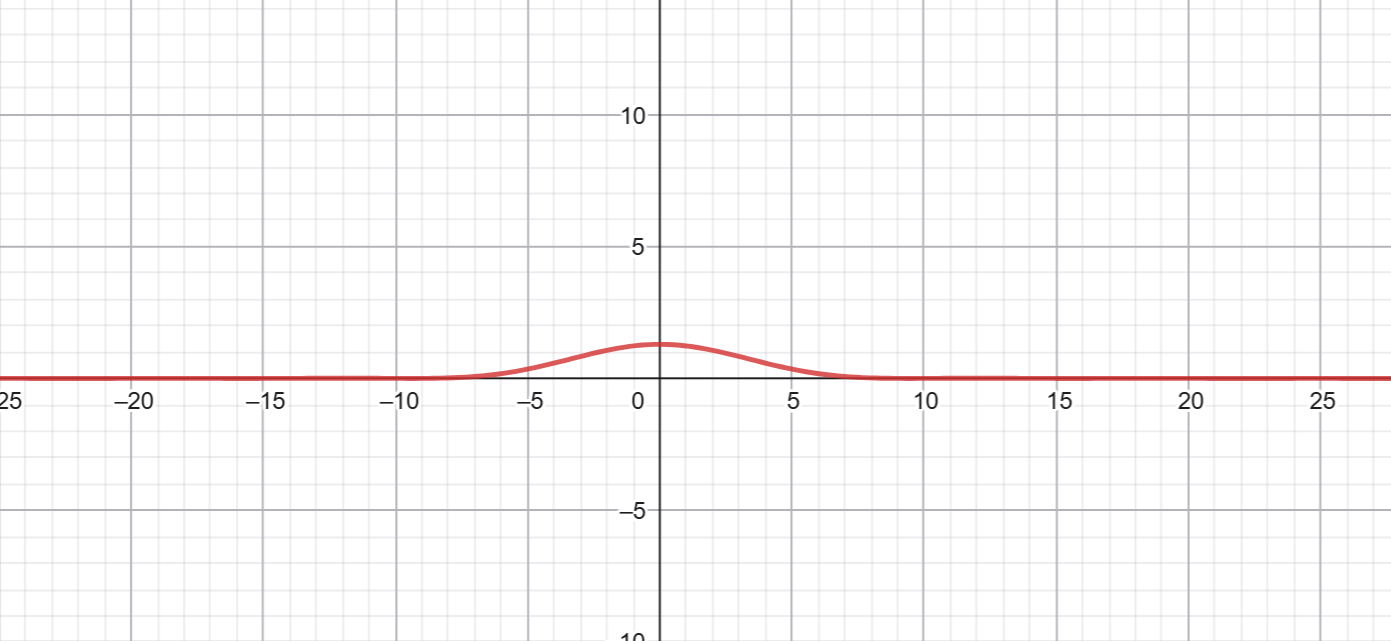
\includegraphics[width=0.8\textwidth,valign=t]{fig/prob3.34n1.png}
        \item $n=2$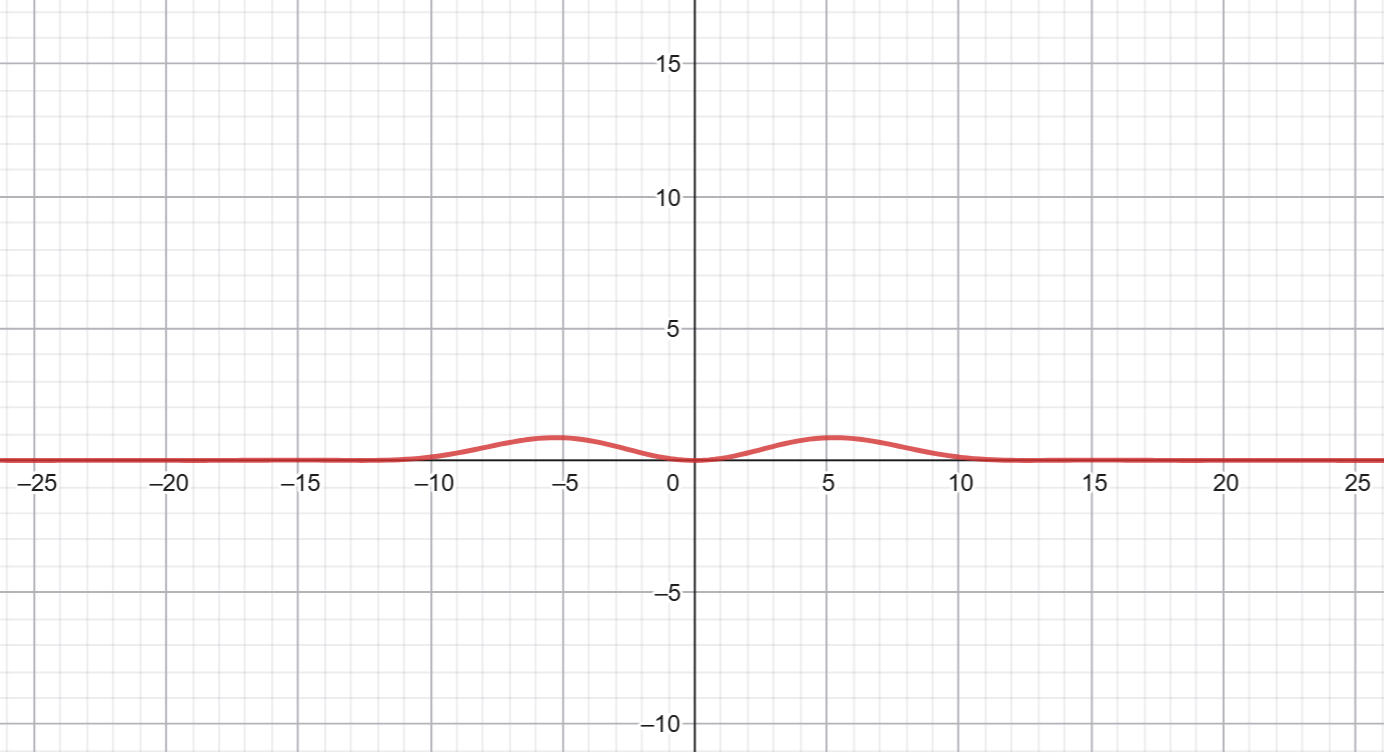
\includegraphics[width=0.8\textwidth, valign=t]{fig/prob3.34n2.png}
    \item $n=5$ 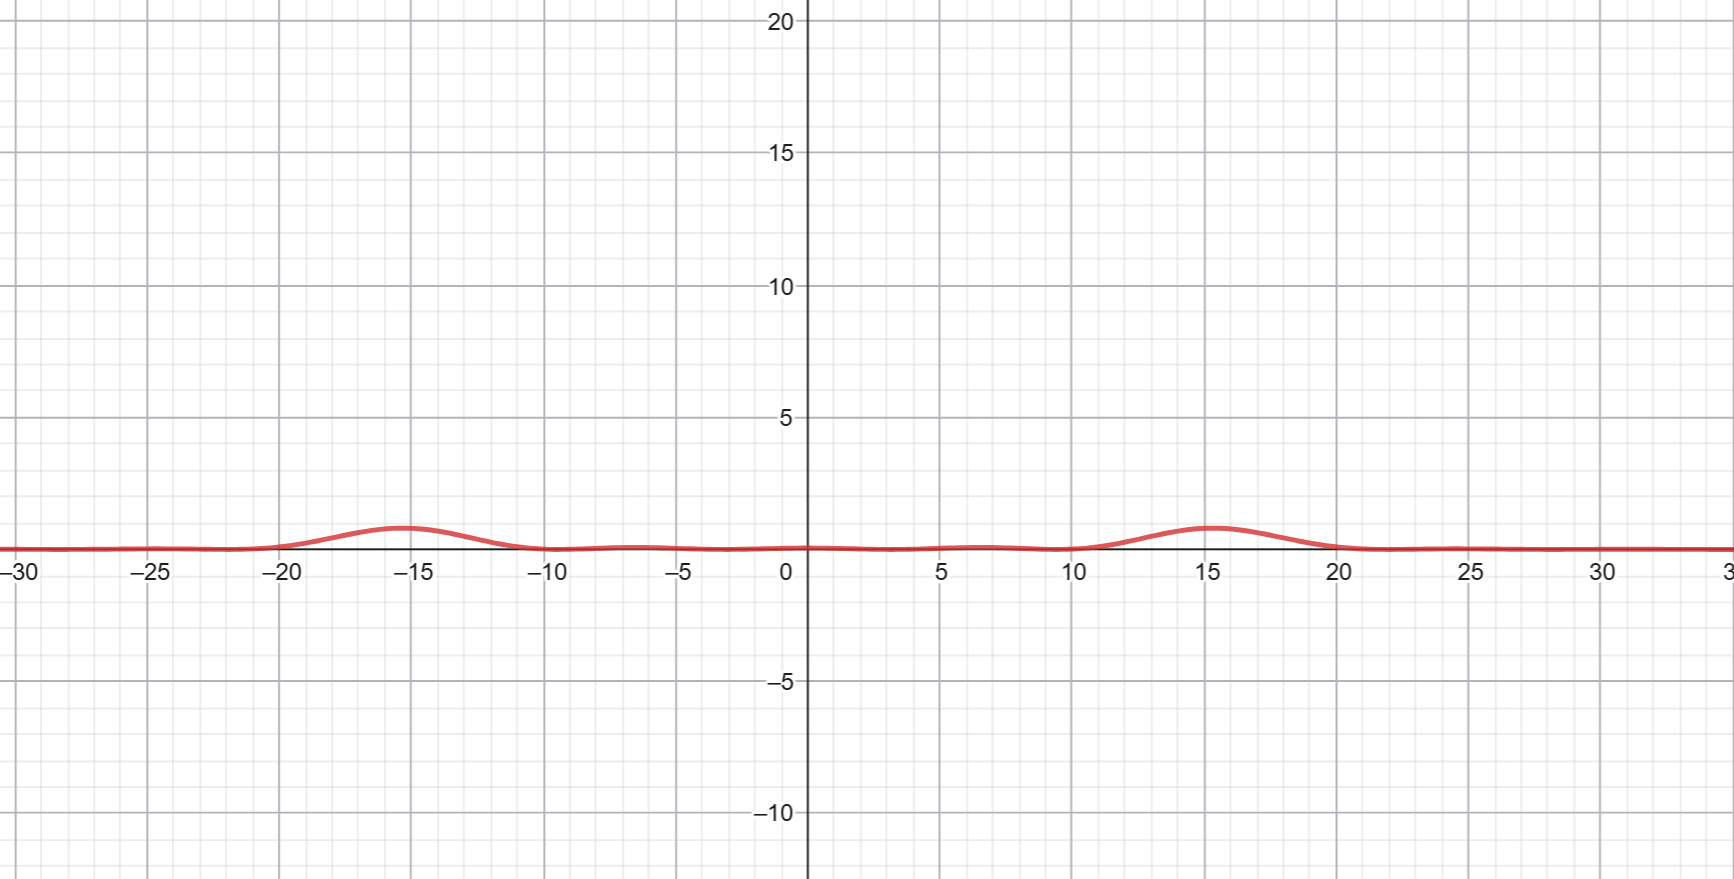
\includegraphics[width=0.8\textwidth, valign=t]{fig/prob3.34n5.png}
    \item $n=10$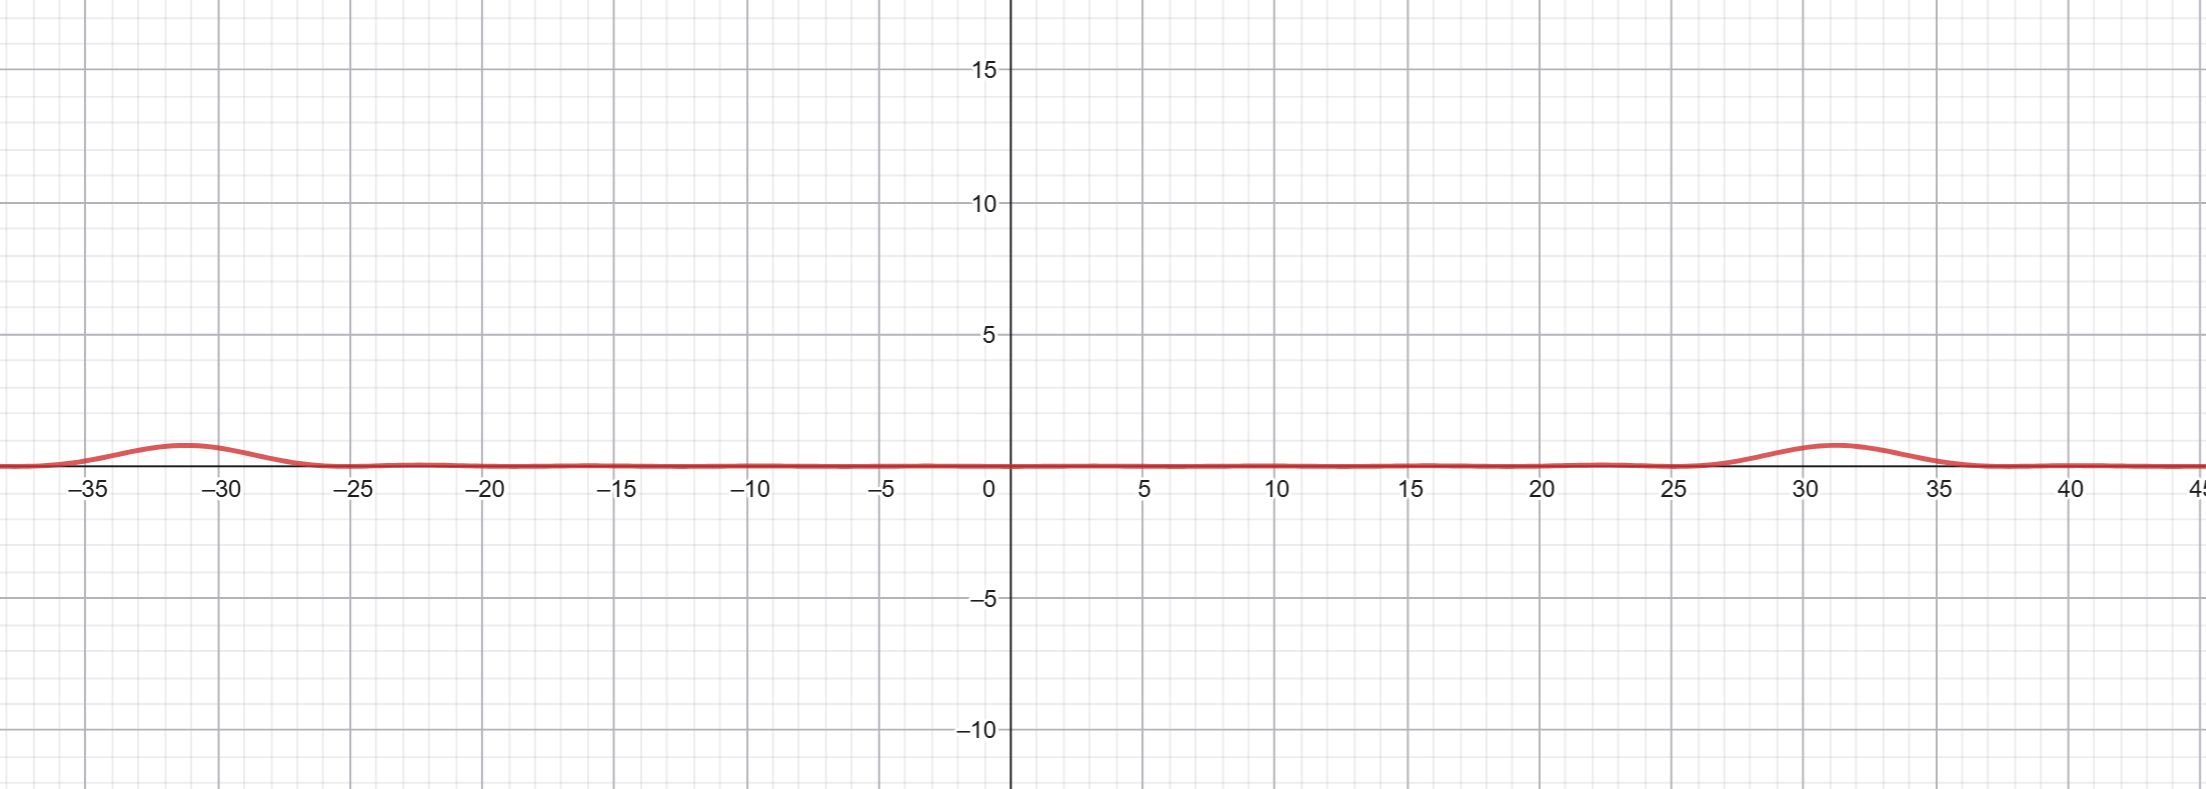
\includegraphics[width=0.8\textwidth, valign=t]{fig/prob3.34n10.png}
    \end{itemize}
    
    For large $n,$ the most probable values are $p=\pm\frac{n\pi\hbar}{a}.$

    For large $n,$ it behaves more like a classical particle. So $\frac{p^2}{2m}=E_n=\frac{n^2\pi^2\hbar^2}{2ma^2},$ the momentum is likely to be $\frac{n\pi\hbar}{a}.$ 

    In prob3.10, we observe that the ground state of the infinite square well is not an eigenvector of the momentum operator. However for large $n,$ the possible values concentrate on only two numbers, and the states, although not exactly, behave as if the eigenvectors of the momentum operator.

    \item 
    \begin{align*}
        \langle p^2\rangle=&
        \int_{-\infty}^{\infty} p^2\frac{1}{a\pi\hbar}
        \left(\frac{\pi n/a}{\pi^2n^2/a^2-p^2/\hbar^2}\right)^2
        2\left(1-(-1)^n\cos\frac{pa}{\hbar}\right) dp\\
        =&
        \frac{2}{a\pi\hbar}
        \frac{\pi^2n^2}{a^2}
        \int_{-\infty}^{\infty}
        \left(
        \frac{p}{\pi^2n^2/a^2-p^2/\hbar^2}
        \right)^2
        (1-(-1)^n\cos\frac{pa}{\hbar})dp
    \end{align*}
    This integration is far too complex. After doing some research, I confirmed that the result is as same as prob2.4, $\langle p^2\rangle=\frac{n^2\pi^2\hbar^2}{a^2}.$
    
\end{enumerate}

\subsection*{Sol. 35}
\begin{align*}
    \Phi(p,0)=&
    \frac{1}{\sqrt{2\pi\hbar}}
    \int_{-n\lambda}^{n\lambda}
    e^{-ipx/\hbar}
    \frac{1}{\sqrt{2n\lambda}}
    e^{i2\pi x/\lambda}dx
    \\=&
     \frac{1}{\sqrt{2\pi\hbar}}
     \frac{1}{\sqrt{2n\lambda}}
     \frac{1}{\frac{-ip}{\hbar}+\frac{2\pi i}{\lambda}}
     (e^{(2\pi i/\lambda-ip/\hbar)n\lambda}-e^{-(2\pi i/\lambda-ip/\hbar)n\lambda})\\
     =&\frac{1}{\sqrt{\pi\hbar n\lambda}}\frac{\lambda\hbar}{p\lambda-2\pi \hbar}\sin\left(\frac{pn\lambda}{\hbar}\right)
\end{align*}
\begin{align*}
    |\Psi(x,0)|^2 = \frac{1}{2n\lambda}, \; -n\lambda < x<n\lambda
\end{align*}
\begin{align*}
    |\Phi(p,0)|^2 = 
    \frac{1}{\pi n}\frac{\lambda\hbar}{(p\lambda-2\pi \hbar)^2}
    \sin^2\left(\frac{pn\lambda}{\hbar}\right)
\end{align*}
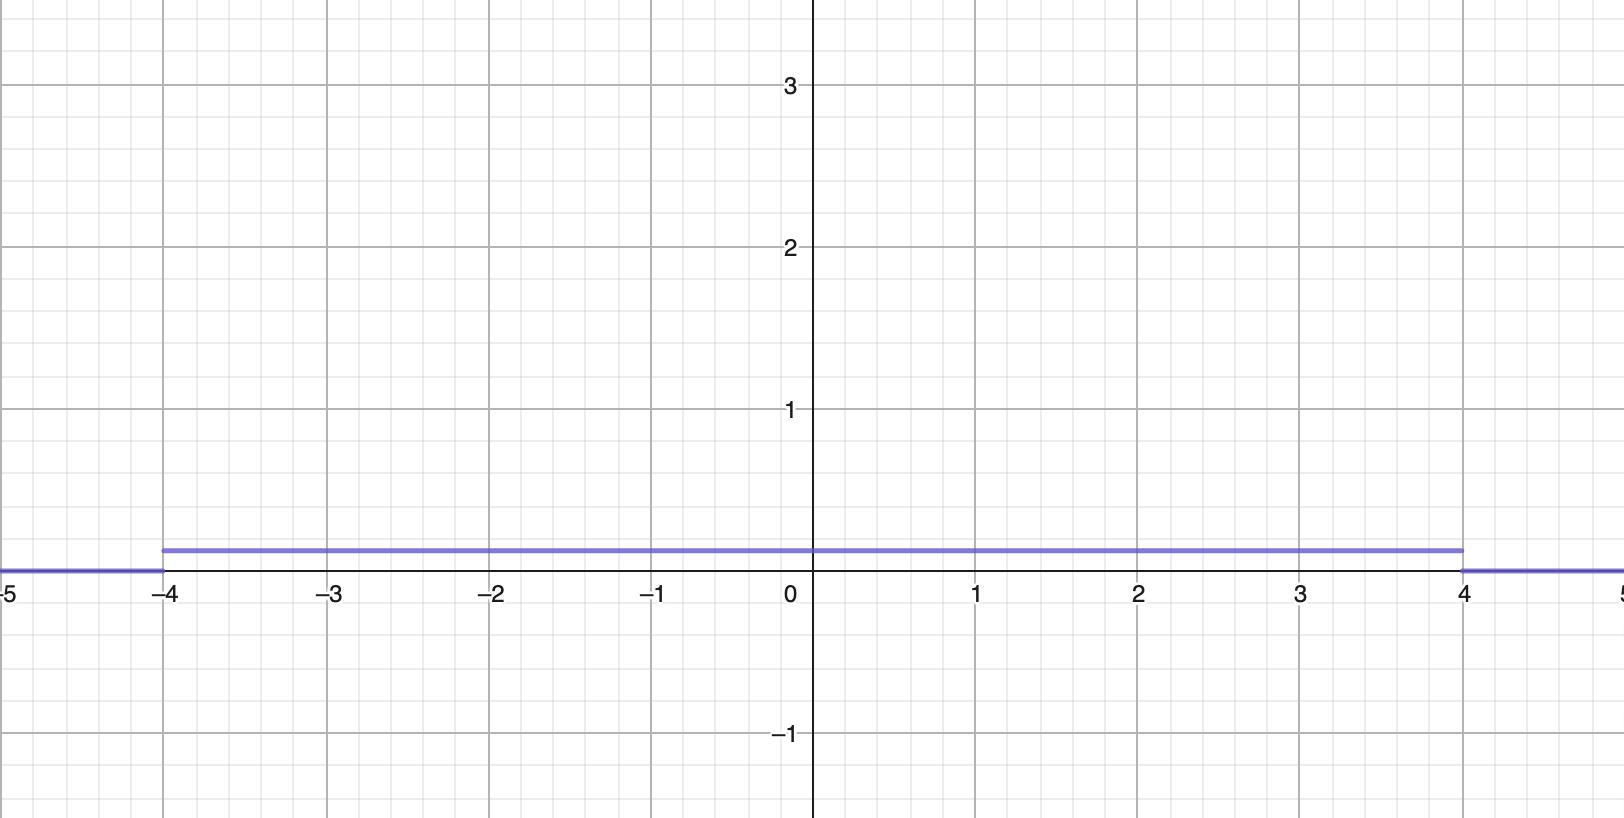
\includegraphics[width=0.8\textwidth, valign=t]{fig/prob3.35x.png}

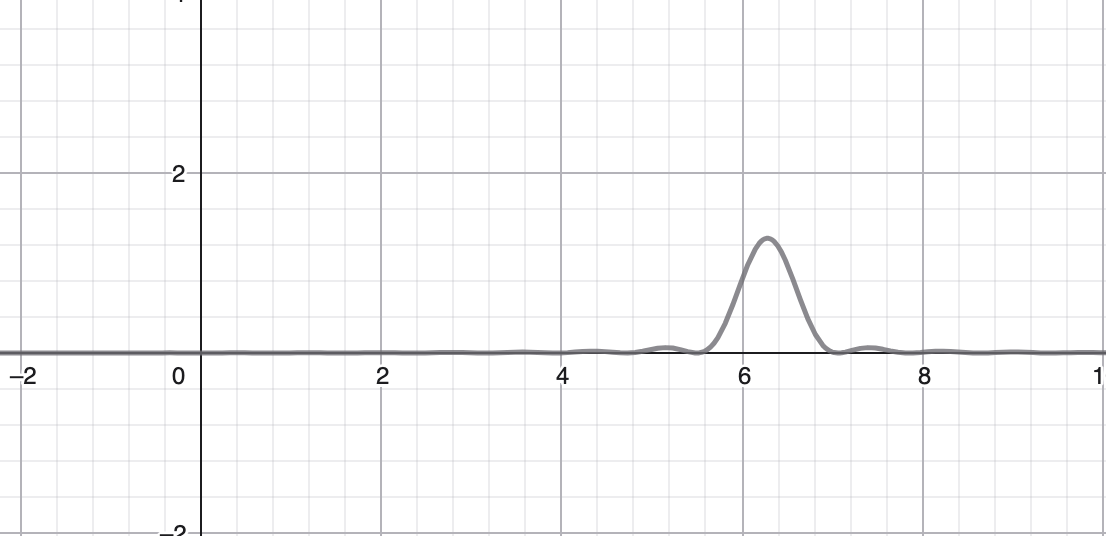
\includegraphics[width=0.8\textwidth, valign=t]{fig/prob3.35p.png}

$$
w_x = 2n\lambda
$$
$$
w_p = \frac{2\pi \hbar}{n\lambda}
$$
As $n\to\infty,$ $w_x\to\infty,$ $w_p\to0.$
$$
w_xw_p = 4\pi\hbar \geq \frac{\hbar}{2}
$$

\begin{align*}
    \langle p\rangle
=&\int_{-n\lambda}^{n\lambda}
\frac{1}{\sqrt{2n\lambda}}e^{-i2\pi x/\lambda}
(-i\hbar\frac{d}{dx})
\frac{1}{\sqrt{2n\lambda}}e^{i2\pi x/\lambda}dx\\
=&\frac{-i\hbar}{2n\lambda}
\int_{-n\lambda}^{n\lambda}
e^{-i2\pi x/\lambda}(i2\pi/\lambda)e^{i2\pi x/\lambda}dx\\
=&\frac{2\pi\hbar}{\lambda}
\end{align*}

\begin{align*}
    \langle p^2\rangle
=&\int_{-n\lambda}^{n\lambda}
\frac{1}{\sqrt{2n\lambda}}e^{-i2\pi x/\lambda}
(-\hbar^2\frac{d^2}{dx^2})
\frac{1}{\sqrt{2n\lambda}}e^{i2\pi x/\lambda}dx\\
=&\frac{-\hbar^2}{2n\lambda}
\int_{-n\lambda}^{n\lambda}
e^{-i2\pi x/\lambda}(i2\pi/\lambda)^2e^{i2\pi x/\lambda}dx\\
=&\frac{4\pi^2\hbar^2}{\lambda^2}
\end{align*}

$\sigma_p=0.$ The abrupt cutoff at the endpoints makes this result not reliable. It hides a delta function when momentum operator is applied.

\subsection*{Sol. 36}
\begin{enumerate}
    \item 
    \begin{align*}
        \int_{-\infty}^{\infty}
        \frac{A^2}{(x^2+a^2)^2}dx = \frac{\pi A^2}{2a^3}.
    \end{align*}
    $$
    A = \sqrt{\frac{2a^3}{\pi}}.
    $$
    \item 
    \begin{align*}
        \langle x\rangle
        =
        \frac{2a^3}{\pi}\int_{-\infty}^{\infty} \frac{x}{(x^2+a^2)^2}dx=0
    \end{align*}
    \begin{align*}
        \langle x^2\rangle
        =
        \frac{2a^3}{\pi}\int_{-\infty}^{\infty} \frac{x^2}{(x^2+a^2)^2}dx=a
    \end{align*}
    $$
    \sigma_x=\sqrt{a}
    $$
    \item 
    \begin{align*}
        \Phi(p,0)
        =&
        \frac{1}{\sqrt{2\pi\hbar}}
        \int_{-\infty}^{\infty}
        e^{-ipx/\hbar}
        \sqrt{\frac{2a^3}{\pi}}
        \frac{1}{x^2+a^2}dx\\
        =&\sqrt{\frac{a}{\hbar}}e^{-\frac{a|p|}{\hbar}}
    \end{align*}
    \begin{align*}
        \int_{-\infty}^{\infty}
        \frac{a}{\hbar}e^{-\frac{2a|p|}{\hbar}}dp = 1
    \end{align*}
    \item 
    \begin{align*}
        \langle p\rangle
        =\int_{-\infty}^{\infty}
        \frac{a}{\hbar}pe^{-\frac{2a|p|}{\hbar}}dp= 0
    \end{align*}
    \begin{align*}
        \langle p^2\rangle
        =\int_{-\infty}^{\infty}
        \frac{a}{\hbar}p^2e^{-\frac{2a|p|}{\hbar}}dp= \frac{\hbar^2}{2a^2}
    \end{align*}
    $$
    \sigma_p = \frac{\hbar}{\sqrt{2}a}
    $$
    \item 
    $$
    \sigma_x\sigma_p=\frac{\hbar}{\sqrt{2}}\geq \frac{\hbar}{2}
    $$
\end{enumerate}

\subsection*{Sol. 37}
\begin{align*}
    \frac{d}{dt}\langle xp\rangle
    =&\frac{i}{\hbar}
    \langle[H,xp]\rangle\\
    =&\frac{i}{\hbar}
    \langle[T+V,xp]\rangle\\
    =&\frac{i}{\hbar}
    \langle x[V,p]+[T,x]p\rangle)\\
    =&\frac{i}{\hbar}
    \langle i\hbar x\frac{\partial V}{\partial x}+\frac{-i\hbar}{m}p^2\rangle\\
    =&2\langle T\rangle-\langle x\frac{\partial V}{\partial x}\rangle.
\end{align*}
There is no $t$ term in the stationary state, so
$$
2\langle T\rangle=\langle x\frac{d V}{d x}\rangle.
$$
For a harmonic oscillator, $V=\frac{1}{2}m\omega^2x^2,$
$$
2\langle T \rangle = \langle xm\omega^2x\rangle\Rightarrow
\langle T\rangle=\langle V\rangle.
$$

\subsection*{Sol. 38}
$$
\Psi(x,t) = 
\frac{1}{\sqrt{2}}\psi_1(x)e^{-iE_1t/\hbar} +
\frac{1}{\sqrt{2}}\psi_2(x)e^{-iE_2t/\hbar}
$$

\begin{align*}
    &\int 
    \left(\frac{1}{\sqrt{2}}\psi_1(x) +
\frac{1}{\sqrt{2}}\psi_2(x)\right)
    \left(\frac{1}{\sqrt{2}}\psi_1(x)e^{-iE_1\tau/\hbar} +
\frac{1}{\sqrt{2}}\psi_2(x)e^{-iE_2\tau/\hbar}\right)dx\\
=&
\frac{1}{2}e^{-iE_1\tau/\hbar}
+\frac{1}{2}e^{-iE_2\tau/\hbar}=0
\end{align*}
$$
\frac{E_2\tau}{\hbar}-\frac{E_1\tau}{\hbar}=\pi 
\Rightarrow\tau=\frac{\pi\hbar}{E_2-E_1}
$$

$$
\Delta H = \sqrt{\frac{1}{2}(E_1^2+E_2^2)-\frac{1}{4}(E_1+E_2)^2}
$$

$$
\Delta H\Delta t
=
\hbar\sqrt{\frac{\frac{1}{2}(E_1^2+E_2^2)-\frac{1}{4}(E_1+E_2)^2}{(E_2-E_1)^2}} = \frac{\hbar}{2}
$$
\subsection*{Sol. 39}

\begin{align*}
    \langle n,xn'\rangle
    =& \left\langle \frac{1}{\sqrt{n!}}
    a_+^n\psi_0,
    x\frac{1}{\sqrt{n'!}}a_+^{n'}\psi_0\right\rangle\\
    =&
    \frac{1}{\sqrt{n!}}
    \frac{1}{\sqrt{n'!}}
    \sqrt{\frac{\hbar}{2m\omega}}
    \langle \psi_0, (a_-)^{n}(a_++a_-)(a_+)^{n'}\psi_0\rangle\\
    =&\frac{1}{\sqrt{n!}}
    \frac{1}{\sqrt{n'!}}
    \sqrt{\frac{\hbar}{2m\omega}}
    (\langle \psi_0, (a_-)^{n}(a_+)^{n'+1}\psi_0\rangle
    +\langle \psi_0, (a_-)^{n+1}(a_+)^{n'}\psi_0\rangle
    )\\
    =&\sqrt{\frac{\hbar}{2m\omega}}(\sqrt{n}\delta_{n-1,n'}+\sqrt{n'}\delta_{n,n'-1})
\end{align*}


\begin{align*}
    \langle n,pn'\rangle
    =& \left\langle \frac{1}{\sqrt{n!}}
    a_+^n\psi_0,
    p\frac{1}{\sqrt{n'!}}a_+^{n'}\psi_0\right\rangle\\
    =&
    \frac{1}{\sqrt{n!}}
    \frac{1}{\sqrt{n'!}}
    i\sqrt{\frac{\hbar m\omega}{2}}
    \langle \psi_0, (a_-)^{n}(a_+-a_-)(a_+)^{n'}\psi_0\rangle\\
    =&\frac{1}{\sqrt{n!}}
    \frac{1}{\sqrt{n'!}}
    i\sqrt{\frac{\hbar m\omega}{2}}
    (\langle \psi_0, (a_-)^{n}(a_+)^{n'+1}\psi_0\rangle
    -\langle \psi_0, (a_-)^{n+1}(a_+)^{n'}\psi_0\rangle
    )\\
    =& i\sqrt{\frac{\hbar m\omega}{2}}(\sqrt{n}\delta_{n-1,n'}-\sqrt{n'}\delta_{n,n'-1})
\end{align*}


\begin{align*}
    X^2_{jk} =&
    \sum_{l}X_{jl}X_{lk}\\
    =&\frac{\hbar}{2m\omega}
    \sum_{l}
    (\sqrt{j}\delta_{j-1,l}+\sqrt{l}\delta_{j,l-1})
    (\sqrt{l}\delta_{l-1,k}+\sqrt{k}\delta_{l,k-1})\\
    =&\frac{\hbar}{2m\omega}
    (\sqrt{j}
    (\sqrt{j-1}\delta_{j-1,k}+
    \sqrt{k}\delta_{j-1,k-1})
    +
    \sqrt{j+1}
    (\sqrt{j+1}\delta_{j,k}+
    \sqrt{k}\delta_{j+1,k-1})\\
    &+
    (\sqrt{j}\delta_{j-1,k+1}+
    \sqrt{k+1}\delta_{j,k})\sqrt{k+1}+
    (\sqrt{j}\delta_{j-1,k-1}+
    \sqrt{k-1}\delta_{j,k-2})\sqrt{k}
    )
\end{align*}
\begin{align*}
    P^2_{jk} =&
    \sum_{l}P_{jl}P_{lk}\\
    =&-\frac{\hbar m\omega}{2}
    \sum_{l}
    (\sqrt{j}\delta_{j-1,l}-\sqrt{l}\delta_{j,l-1})
    (\sqrt{l}\delta_{l-1,k}-\sqrt{k}\delta_{l,k-1})\\
    =&-\frac{\hbar m\omega}{2}
    (\sqrt{j}
    (\sqrt{j-1}\delta_{j-1,k}-
    \sqrt{k}\delta_{j-1,k-1})
    -
    \sqrt{j+1}
    (\sqrt{j+1}\delta_{j,k}-
    \sqrt{k}\delta_{j+1,k-1})\\
    &+
    (\sqrt{j}\delta_{j-1,k+1}-
    \sqrt{k+1}\delta_{j,k})\sqrt{k+1}-
    (\sqrt{j}\delta_{j-1,k-1}-
    \sqrt{k-1}\delta_{j,k-2})\sqrt{k}
    )
\end{align*}

\begin{align*}
    \frac{1}{2m}P^2_{jk}
    +\frac{m\omega^2}{2}X^2_{jk}
    =&\frac{\hbar\omega}{4}
    2(\sqrt{kj}\delta_{j,k}+(j+1)\delta_{j,k}+(k+1)\delta_{j,k}+\sqrt{jk}\delta_{j,k})\\
    =&\frac{\hbar\omega}{2}(2j+1)\delta_{j,k}
\end{align*}

\subsection*{Sol. 40}
\begin{align*}
    \langle x\rangle = &
    \sum_{n,s}c_s^*e^{iE_nt/\hbar}
    c_ne^{-iE_st/\hbar}\langle\psi_s, x\psi_n\rangle\\
    =&\sqrt{\frac{\hbar}{2m\omega}}\sum_{n,s}
    c_s^*c_ne^{iE_nt/\hbar}
    e^{-iE_st/\hbar}(\sqrt{n}\delta_{s,n-1}+\sqrt{s}\delta_{s-1,n})\\
    =&\sqrt{\frac{\hbar}{2m\omega}}\sum_n(
    c_{n+1}^*c_ne^{iE_nt/\hbar}
    e^{-iE_{n+1}t/\hbar}\sqrt{n+1}
    +c_{n-1}^*c_ne^{iE_nt/\hbar}
    e^{-iE_{n-1}t/\hbar}\sqrt{n})\\
    =&\sqrt{\frac{\hbar}{2m\omega}}\sum_n
    \sqrt{n+1}
    (c^*_{n+1}c_ne^{-i\omega t}+c^*_{n}c_{n+1}e^{i\omega t})
\end{align*}
Let $$
Ce^{i\phi} = 
\sqrt{\frac{2\hbar}{m\omega}}\sum_n
    \sqrt{n+1}
    c^*_{n+1}c_n,
$$ then 
$$
\langle x\rangle
=\frac{1}{2}Ce^{i\phi}e^{-i\omega t} + \frac{1}{2}Ce^{-i\phi} e^{i\omega t} = C\cos(\omega t-\phi).
$$

For problem 2.40, $c_0=\frac{3}{5},$ $c_1=-\frac{2\sqrt{2}}{5},$ $c_2=\frac{2\sqrt{2}}{5}.$
$$
\phi=0,
$$
$$
C = \sqrt{\frac{2\hbar}{m\omega}}
(\sqrt{1}c_1c_0+\sqrt{2}c_2c_1)
= \sqrt{\frac{2\hbar}{m\omega}}
(-\frac{14\sqrt{2}}{25}).
$$


\subsection*{Sol. 41}
$$
\Psi(x,t) = \frac{1}{\sqrt{2}}\psi_0e^{-iE_0t/\hbar}
+
\frac{1}{\sqrt{2}}\psi_1e^{-iE_1t/\hbar}
$$

\begin{align*}
    \langle p\rangle =& 
    \langle \frac{1}{\sqrt{2}}\psi_0e^{-iE_0t/\hbar}
+
\frac{1}{\sqrt{2}}\psi_1e^{-iE_1t/\hbar}, p(\frac{1}{\sqrt{2}}\psi_0e^{-iE_0t/\hbar}
+
\frac{1}{\sqrt{2}}\psi_1e^{-iE_1t/\hbar})\rangle\\
=&\frac{1}{2}e^{iE_0 t/\hbar}e^{-iE_1 t/\hbar}\langle \psi_0, p\psi_1\rangle
+\frac{1}{2}e^{-iE_0 t/\hbar}e^{iE_1 t/\hbar}\langle \psi_1, p\psi_0\rangle\\
=&
\frac{1}{2}e^{iE_0 t/\hbar}e^{-iE_1 t/\hbar}
(-i\sqrt{\frac{\hbar m\omega}{2}})
+\frac{1}{2}e^{-iE_0 t/\hbar}e^{iE_1 t/\hbar} 
(i\sqrt{\frac{\hbar m\omega}{2}})\\
=&-\sqrt{\frac{\hbar m\omega}{2}}\sin\omega t
\end{align*}
The largest value of $\langle p\rangle$ is $\sqrt{\frac{\hbar m\omega}{2}}.$

\subsection*{Sol. 42}
\begin{enumerate}
    \item 
    \begin{align*}
        \langle x\rangle
        =&
        \sqrt{\frac{\hbar}{2m\omega}}
        \langle \alpha, (a_++a_-)\alpha\rangle\\
        =&\sqrt{\frac{\hbar}{2m\omega}}
        (\langle a_-\alpha,\alpha\rangle + \langle\alpha,a_-,\alpha\rangle)\\
        =&
        \sqrt{\frac{\hbar}{2m\omega}}
        (\bar{\alpha}+\alpha)
    \end{align*}
    \begin{align*}
        \langle x^2\rangle
        =&
        \frac{\hbar}{2m\omega}
        \langle \alpha, (a_++a_-)^2\alpha\rangle\\
        =&\frac{\hbar}{2m\omega}
        (\langle\alpha, a_+^2\alpha\rangle+
        \langle\alpha, a_+a_-\alpha\rangle
        +
        \langle\alpha, a_-a_+\alpha\rangle+
        \langle\alpha, a_-^2\alpha\rangle)\\
        =&\frac{\hbar}{2m\omega}
        (\langle a_-^2\alpha, \alpha\rangle+
        \langle a_-\alpha, a_-\alpha\rangle
        +
        \langle\alpha, (1+a_+a_-)\alpha\rangle+
        \langle\alpha, a_-^2\alpha\rangle)\\
        =&
        \frac{\hbar}{2m\omega}
        (\bar{\alpha}^2+\alpha^2+2\bar{\alpha}\alpha + 1
        )
    \end{align*}
    \begin{align*}
        \langle p\rangle
        =&
        i
        \sqrt{\frac{\hbar m\omega}{2}}
        \langle \alpha, (a_+-a_-)\alpha\rangle\\
        =&i
        \sqrt{\frac{\hbar m\omega}{2}}
        (\langle a_-\alpha,\alpha\rangle -\langle\alpha,a_-,\alpha\rangle)\\
        =&
        i
        \sqrt{\frac{\hbar m\omega}{2}}
        (\bar{\alpha}-\alpha)
    \end{align*}
    \begin{align*}
        \langle p^2\rangle
        =&
        -\frac{\hbar m\omega}{2}
        \langle \alpha, (a_+-a_-)^2\alpha\rangle\\
        =&-\frac{\hbar m\omega}{2}
        (\langle\alpha, a_+^2\alpha\rangle-
        \langle\alpha, a_+a_-\alpha\rangle
        -
        \langle\alpha, a_-a_+\alpha\rangle+
        \langle\alpha, a_-^2\alpha\rangle)\\
        =&-\frac{\hbar m\omega}{2}
        (\langle a_-^2\alpha, \alpha\rangle
        -
        \langle a_-\alpha, a_-\alpha\rangle
        -
        \langle\alpha, (1+a_+a_-)\alpha\rangle+
        \langle\alpha, a_-^2\alpha\rangle)\\
        =&
        -\frac{\hbar m\omega}{2}
        (\bar{\alpha}^2-2\bar{\alpha}\alpha - 1 + \alpha^2
        )
    \end{align*}
    \item 
    $$
    \sigma_x= 
    \sqrt{\frac{\hbar}{2m\omega}}
    $$
    $$
    \sigma_p = 
    \sqrt{\frac{\hbar m\omega}{2}}
    $$
    $$
    \sigma_x\sigma_p=\frac{\hbar}{2}
    $$
    \item 
    $$
    \sum_{n=0}c_na_-| n\rangle = 
    \sum_{n=0}c_n\sqrt{n}|n-1\rangle
    =
    \sum_{n=0}c_{n+1}\sqrt{n+1}|n\rangle
    =\alpha\sum_{n=0}c_n| n\rangle
    $$
    Thus, $$c_{n+1}\sqrt{n+1}=\alpha c_n
    \Rightarrow
    c_n = \frac{\alpha^n}{\sqrt{n!}}c_0.
    $$ 
    \item 
    \begin{align*}
        \sum_{n=0}\frac{|\alpha|^{2n}}{n!}|c_0|^2=
        |c_0|^2e^{|\alpha|^2}\Rightarrow c_0=e^{-|\alpha|^2/2}\\
    \end{align*}
    \item 
    \begin{align*}
        a_-|\alpha(t)\rangle =&
        a_-\sum_{n=0} \frac{\alpha^n}{\sqrt{n!}}c_0e^{-i\omega(2n+1)t/2}|n\rangle\\
        =&\sum_{n=1} \frac{\alpha^n}{\sqrt{(n-1)!}}c_0e^{-i\omega(2n+1)t/2}|n-1\rangle
        \\
        =&\sum_{n=0} \frac{\alpha^{n+1}}{\sqrt{n!}}c_0e^{-i\omega(2n+3)t/2}|n\rangle\\
        =&\alpha e^{-i\omega t}|\alpha(t)\rangle
    \end{align*}
    \item 
    \begin{align*}
        \langle x\rangle
        =&\sqrt{\frac{\hbar}{2m\omega}}
        (e^{i\omega t}\bar{\alpha} + e^{-i\omega t}\alpha)\\
        =&C\cos(\omega t-\phi)
    \end{align*}
    $$
    \sigma_x = \sqrt{\frac{\hbar}{2m\omega}}
    $$
    \item 
    Yes. Since $a_-\psi_0=0\cdot\psi_0,$ the eigenvalue is 0.
\end{enumerate}

\subsection*{Sol. 43}
\begin{enumerate}
    \item 
    By equation 3.59, 
    $$
    \sigma_A^2\sigma_B^2\geq |\langle AB\rangle-\langle A\rangle\langle B\rangle|^2
    $$

    \begin{align*}
        \frac{1}{4}(\langle C\rangle^2+\langle D\rangle^2)
    =&
    \frac{1}{4}
    (\langle -i(AB-BA)\rangle^2 + \langle AB+BA-2\langle A\rangle\langle B\rangle\rangle^2)\\
    =&
    \frac{1}{4}
    (\langle -i(AB-BA)\rangle^2 + \langle AB+BA-2\langle A\rangle\langle B\rangle\rangle^2)\\
    =&
    \frac{1}{4}
    (-\langle AB\rangle^2+2\langle AB\rangle\langle BA\rangle
    -\langle BA\rangle^2
    + \langle AB\rangle^2 
    + \langle BA\rangle^2\\
    &+ 4\langle A\rangle^2\langle B\rangle^2
    + 2\langle AB\rangle\langle BA\rangle
    -2\langle AB\rangle\langle A\rangle\langle B\rangle
    -2\langle BA\rangle\langle A\rangle\langle B\rangle
    )\\
    =&
    \frac{1}{4}(4\langle AB\rangle\langle BA\rangle+
    4\langle A\rangle^2\langle B\rangle^2
    -2\langle AB\rangle\langle A\rangle\langle B\rangle
    -2\langle BA\rangle\langle A\rangle\langle B\rangle
    )\\
    =&|\langle AB\rangle-\langle A\rangle\langle B\rangle|^2
    \end{align*}
    \item If $B=A,$ then
    $$
    \sigma_A^4\geq 
    \frac{1}{4}(\langle 2A^2-2\langle A\rangle^2\rangle^2)
    \Rightarrow 
    \sigma_A^2\geq 
    \langle A^2-\langle A\rangle^2\rangle
    \Rightarrow \sigma_A^2\geq \sigma_A^2.
    $$
\end{enumerate}

\subsection*{Sol. 44}
\begin{enumerate}
    \item 
    \begin{align*}
        det(H-tI)=&
    (a-t)(c-t)(a-t) - b^2(c-t)\\
    =&(c-t)(a^2-2at+t^2-b^2)\\
    =&(c-t)(a+b-t)(a-b-t)
    \end{align*}
    Eigenvalues $c: 
    \begin{pmatrix}
    0\\1\\ 0
    \end{pmatrix},
    $
    $a+b: 
    \frac{1}{\sqrt{2}}\begin{pmatrix}
    1\\0\\ 1
    \end{pmatrix},
    $
    $a-b: 
    \frac{1}{\sqrt{2}}
    \begin{pmatrix}
    1\\0\\ -1
    \end{pmatrix}.
    $

    If $|\mathcal{S}(0)\rangle = \begin{pmatrix}
        0\\1\\0
    \end{pmatrix},$ then
    $$
    |\mathcal{S}(t)\rangle
    =
    \begin{pmatrix}
    0\\1\\ 0
    \end{pmatrix}e^{-ict/\hbar}
    $$
    \item 

     If $|\mathcal{S}(0)\rangle = \begin{pmatrix}
        1\\0\\0
    \end{pmatrix},$ then
    $$
    |\mathcal{S}(t)\rangle
    =
    \frac{1}{2}
    \begin{pmatrix}
    1\\0\\ 1
    \end{pmatrix}e^{-i(a+b)t/\hbar}
    +
    \frac{1}{2}
    \begin{pmatrix}
    1\\0\\ -1
    \end{pmatrix}e^{-i(a-b)t/\hbar}.
    $$
    
\end{enumerate}

\subsection*{Sol. 45}
\begin{align*}
    \langle n|\hat{x}|\mathcal{S}(t)\rangle =& 
    \sum_{n'}\langle n|\hat{x}|n'\rangle\langle n'|\mathcal{S}(t)\rangle \\
    =& 
    \sum_{n'}c_{n'}(t)\langle n|\hat{x}|n'\rangle\\
    =&\sqrt{\frac{\hbar}{2m\omega}}
    \sum_{n'}
    c_{n'}(t)
    (\sqrt{n'}\delta_{n,n'-1}
    +\sqrt{n}\delta_{n',n-1}
    )\\
    =&
    \sqrt{\frac{\hbar}{2m\omega}}
    (c_{n+1}(t)\sqrt{n+1}
    +
    c_{n-1}(t)\sqrt{n}
    )
\end{align*}
\subsection*{Sol. 46}

\begin{enumerate}
    \item 
    $H:$
    Eigenvalues: 
    \begin{itemize}
        \item $
    \hbar\omega: 
    \begin{pmatrix}
    1\\0\\0
    \end{pmatrix}
    $
     \item $
    2\hbar\omega: 
    \begin{pmatrix}
    0\\1\\0
    \end{pmatrix}
    $
     \item $
    2\hbar\omega: 
    \begin{pmatrix}
    0\\0\\1
    \end{pmatrix}
    $
    \end{itemize}

     $A:$
    Eigenvalues: 
    \begin{itemize}
        \item $
    2\lambda: 
    \begin{pmatrix}
    0\\0\\1
    \end{pmatrix}
    $
     \item $
    \lambda:
    \frac{1}{\sqrt{2}}
    \begin{pmatrix}
    1\\1\\0
    \end{pmatrix}
    $
     \item $
    -\lambda: 
    \frac{1}{\sqrt{2}}
    \begin{pmatrix}
    1\\-1\\0
    \end{pmatrix}
    $
    
    \end{itemize}
    $B:$
    Eigenvalues: 
    \begin{itemize}
        \item $
    2\mu: 
    \begin{pmatrix}
    1\\0\\0
    \end{pmatrix}
    $
     \item $
    \mu: 
    \frac{1}{\sqrt{2}}
    \begin{pmatrix}
    0\\1\\1
    \end{pmatrix}
    $
     \item $
    -\mu: 
    \frac{1}{\sqrt{2}}
    \begin{pmatrix}
    0\\1\\-1
    \end{pmatrix}
    $
    
    \end{itemize}

    \item 
    $$
    \langle H\rangle
    =
    \begin{pmatrix}
        c_1^* & 
        c_2^* & 
        c_3^*
    \end{pmatrix}
    \hbar\omega
    \begin{pmatrix}
        1 & 0 & 0\\
        0 & 2 & 0\\
        0 & 0 & 2
    \end{pmatrix}
    \begin{pmatrix}
        c_1\\c_2\\c_3
    \end{pmatrix}
    =\hbar\omega
    (|c_1|^2+2|c_2|^2+2|c_3|^2)
    $$
    $$
    \langle A\rangle
    =
    \begin{pmatrix}
        c_1^* & 
        c_2^* & 
        c_3^*
    \end{pmatrix}
    \lambda
    \begin{pmatrix}
        0 & 1 & 0\\
        1 & 0 & 0\\
        0 & 0 & 2
    \end{pmatrix}
    \begin{pmatrix}
        c_1\\c_2\\c_3
    \end{pmatrix}
    =\lambda
    (c_1^*c_2 + c_2^*c_1+2|c_3|^2)
    $$
    $$
    \langle B\rangle
    =
    \begin{pmatrix}
        c_1^* & 
        c_2^* & 
        c_3^*
    \end{pmatrix}
    \mu
    \begin{pmatrix}
        2 & 0 & 0\\
        0 & 0 & 1\\
        0 & 1 & 0
    \end{pmatrix}
    \begin{pmatrix}
        c_1\\c_2\\c_3
    \end{pmatrix}
    =\mu
    (2|c_1|^2+c_2^*c_3+c_3^*c_2)
    $$
    \item 
    $$
    |\mathcal{S}
    (t)
    \rangle
    =
    c_1
    \begin{pmatrix}
        1\\0\\0
    \end{pmatrix}
    e^{-i\omega t}
    +
    c_2
    \begin{pmatrix}
        0\\1\\0
    \end{pmatrix}
    e^{-i2\omega t}
    +
    c_3
    \begin{pmatrix}
        0\\0\\1
    \end{pmatrix}
    e^{-i2\omega t}
    $$

    Measuring $H$ will get $\hbar\omega$ with probability $|c_1|^2,$ and $2\hbar\omega$ with probability $|c_2|^2+|c_3|^2.$

    \begin{align*}
        \langle \mathcal{S}(t)|A|\mathcal{S}(t)\rangle
        =& 
        \left[
         c_1^*
    \begin{pmatrix}
        1&0&0
    \end{pmatrix}
    e^{i\omega t}
    +
    c_2^*
    \begin{pmatrix}
        0&1&0
    \end{pmatrix}
    e^{i2\omega t}
    +
    c_3^*
    \begin{pmatrix}
        0&0&1
    \end{pmatrix}
    e^{i2\omega t}
    \right]
    \lambda
    \begin{pmatrix}
        0 & 1 & 0\\
        1 & 0 & 0\\
        0 & 0 & 2
    \end{pmatrix}\\
    &\left[
    c_1
    \begin{pmatrix}
        1\\0\\0
    \end{pmatrix}
    e^{-i\omega t}
    +
    c_2
    \begin{pmatrix}
        0\\1\\0
    \end{pmatrix}
    e^{-i2\omega t}
    +
    c_3
    \begin{pmatrix}
        0\\0\\1
    \end{pmatrix}
    e^{-i2\omega t}
    \right]\\
    =&
    \left[
         c_1^*
    \begin{pmatrix}
        1&0&0
    \end{pmatrix}
    e^{i\omega t}
    +
    c_2^*
    \begin{pmatrix}
        0&1&0
    \end{pmatrix}
    e^{i2\omega t}
    +
    c_3^*
    \begin{pmatrix}
        0&0&1
    \end{pmatrix}
    e^{i2\omega t}
    \right]
    \lambda
    \\
    &\left[
    c_1
    \begin{pmatrix}
        0\\1\\0
    \end{pmatrix}
    e^{-i\omega t}
    +
    c_2
    \begin{pmatrix}
        1\\0\\0
    \end{pmatrix}
    e^{-i2\omega t}
    +
    c_3
    \begin{pmatrix}
        0\\0\\2
    \end{pmatrix}
    e^{-i2\omega t}
    \right]\\
    =&\lambda(c_1^*c_2e^{-i\omega t}
    +c_2^*c_1e^{i\omega t}
    +|c_3|^2)
    \end{align*}

    \begin{align*}
        \langle \mathcal{S}(t)|B|\mathcal{S}(t)\rangle
        =& 
        \left[
         c_1^*
    \begin{pmatrix}
        1&0&0
    \end{pmatrix}
    e^{i\omega t}
    +
    c_2^*
    \begin{pmatrix}
        0&1&0
    \end{pmatrix}
    e^{i2\omega t}
    +
    c_3^*
    \begin{pmatrix}
        0&0&1
    \end{pmatrix}
    e^{i2\omega t}
    \right]
    \mu
    \begin{pmatrix}
        2 & 0 & 0\\
        0 & 0 & 1\\
        0 & 1 & 0
    \end{pmatrix}\\
    &\left[
    c_1
    \begin{pmatrix}
        1\\0\\0
    \end{pmatrix}
    e^{-i\omega t}
    +
    c_2
    \begin{pmatrix}
        0\\1\\0
    \end{pmatrix}
    e^{-i2\omega t}
    +
    c_3
    \begin{pmatrix}
        0\\0\\1
    \end{pmatrix}
    e^{-i2\omega t}
    \right]\\
    =&
    \left[
         c_1^*
    \begin{pmatrix}
        1&0&0
    \end{pmatrix}
    e^{i\omega t}
    +
    c_2^*
    \begin{pmatrix}
        0&1&0
    \end{pmatrix}
    e^{i2\omega t}
    +
    c_3^*
    \begin{pmatrix}
        0&0&1
    \end{pmatrix}
    e^{i2\omega t}
    \right]
    \mu
    \\
    &\left[
    c_1
    \begin{pmatrix}
        2\\0\\0
    \end{pmatrix}
    e^{-i\omega t}
    +
    c_2
    \begin{pmatrix}
        0\\0\\1
    \end{pmatrix}
    e^{-i2\omega t}
    +
    c_3
    \begin{pmatrix}
        0\\1\\0
    \end{pmatrix}
    e^{-i2\omega t}
    \right]\\
    =&\mu(2|c_1|^2+
    +c_2^*c_3
    +c_3^*c_2)
    \end{align*}
    
\end{enumerate}

\subsection*{Sol. 47}
\begin{enumerate}
    \item 
    \begin{align*}
        A^\dagger A
        =&(-i\frac{p}{\sqrt{2m}}+W)
        (i\frac{p}{\sqrt{2m}}+W)\\
        =&\frac{p^2}{2m}
        -i\frac{pW}{\sqrt{2m}}
        +i\frac{Wp}{\sqrt{2m}}+W^2\\
        =&\frac{p^2}{2m}
            +\frac{i}{\sqrt{2m}}[W,p]+W^2
        \\
        =&\frac{p^2}{2m}+W^2-\frac{\hbar}{\sqrt{2m}}W'
    \end{align*}
    \begin{align*}
        A A^\dagger
        =&
        (i\frac{p}{\sqrt{2m}}+W)
        (-i\frac{p}{\sqrt{2m}}+W)\\
        =&\frac{p^2}{2m}
        +i\frac{pW}{\sqrt{2m}}
        -i\frac{Wp}{\sqrt{2m}}+W^2\\
        =&\frac{p^2}{2m}
            -\frac{i}{\sqrt{2m}}[W,p]+W^2
        \\
        =&\frac{p^2}{2m}+W^2+\frac{\hbar}{\sqrt{2m}}W'
    \end{align*}

    $$
    V_1=W^2-\frac{\hbar}{\sqrt{2m}}W'
    $$
    $$
    V_2=W^2+\frac{\hbar}{\sqrt{2m}}W'
    $$
    \item 
    $$
    H_2A\psi_n^{(1)}
    =AA^\dagger A\psi_n^{(1)}
    =E_n^{(1)}A\psi_n^{(1)}
    $$
     $$
    H_1A^\dagger\psi_n^{(2)}
    =A^\dagger A A^\dagger\psi_n^{(2)}
    =E_n^{(2)}A^\dagger\psi_n^{(2)}
    $$
    \item 
    $$
    i\frac{p}{\sqrt{2m}}\psi_0^{(1)}+W
    \psi_0^{(1)} = 0
    \Rightarrow 
    W=\frac{-\hbar\psi_0^{(1)'}}{\sqrt{2m}\psi_0^{(1)}}
    $$
    \item
    By c,
    $$
    W = \sqrt{\frac{m}{2}}
    \frac{\alpha}{\hbar}
    (\theta(x)-\theta(-x)).
    $$

    By a,
    $$
    V_2 = \frac{m\alpha^2}{2\hbar^2}+\alpha\delta(x).
    $$
\end{enumerate}

\subsection*{Sol. 48}
\begin{enumerate}
    \item 
    \begin{align*}
        \langle g, pf\rangle
    =&\int_0^a\bar{g}(-i\hbar f')\\
    =&\int_0^ai\hbar\bar{g}'f\\
    =&\langle pg,f\rangle
    \Rightarrow p^\dagger = p.
    \end{align*}
    We do not restrict the domain of $p^\dagger,$ so, by definition, it is not self-adjoint. 
    \item 
    \begin{align*}
        \langle g, pf\rangle
    =&\int_0^a\bar{g}(-i\hbar f')\\
    =& -i\hbar (\bar{g}f)\bigg|^a_0+i\hbar \int_0^a\bar{g}'f\\
    =&-i\hbar(\bar{g}(a)f(a)-\bar{g}(0)f(0))+\langle pg, f\rangle\\
    =&
    -i\hbar f(0)(\bar{g}(a)\lambda-\bar{g}(0))+\langle pg, f\rangle
    \end{align*}
    We have to restrict the domain of $p^\dagger$ to those functions that satisfy $g(0)=\bar{\lambda}g(a).$

    If $\lambda$ is selected to be real, then $p$ is self-adjoint.
    \item 
    \begin{align*}
        \langle g, pf\rangle
    =&\int_0^\infty\bar{g}(-i\hbar f')\\
    =& -i\hbar (\bar{g}f)\bigg|^\infty_0+i\hbar \int_0^\infty\bar{g}'f\\
    =&\bar{g}(0)f(0) + \langle pg,f\rangle
    \end{align*}
    Restricting $f(0)$ to be 0 can make $p$ a hermitian operator. The domain of $p^\dagger$ can then be selected 
    to a much bigger set, including those $g(0)\neq 0.$ Therefore, the self-adjoint momentum operator does not exist on this interval.
    
\end{enumerate}
\subsection*{Sol. 49}
\begin{enumerate}
    \item 
    $$
    i\hbar\frac{\partial \Psi}{\partial t}
    =-\frac{\hbar^2}{2m}
    \frac{\partial^2\Psi}{\partial x^2}+V\Psi
    $$
    For a free particle $V=0.$
    Write the Fourier transform as $F,$ and its inverse as $f,$ we have
    $$
    i\hbar D_t f(\Phi)
    =
    -\frac{\hbar^2}{2m}
    D^2f(\Phi)+Vf(\Phi)
    $$

    Note that for any function $g$
    $$
    FD_t(g) = D_tF(g)
    $$

   \begin{align*}
       FD(g) =& \frac{1}{\sqrt{2\pi\hbar}}
    \int e^{-ipx/\hbar}g'\\
    =&\frac{1}{\sqrt{2\pi\hbar}}
    \frac{ip}{\hbar}
    \int e^{-ipx/\hbar}g\\
    =&\frac{ip}{\hbar}F(g),
   \end{align*}
   so 
   \begin{align*}
       FD^2f(\Phi)=&
       i\frac{p}{\hbar}
       FDf(\Phi)\\
       =&-\frac{p^2}{\hbar^2}
       Ff(\Phi)\\
       =&-\frac{p^2}{\hbar^2}\Phi
   \end{align*}
    Thus,
    $$
    i\hbar\frac{\partial\Phi}{\partial t}
     = 
    \frac{p^2}{2m}
    \Phi
    $$
    The solution is 
    $$
    \Phi(p,t)=
    e^{\frac{-ip^2t}{2m\hbar}}\Phi(p,0).
    $$
    \item 
    $$
    \Psi(x,0)=Ae^{-ax^2}e^{ilx}.
    $$
    By normalization, $A^2=\sqrt{\frac{2a}{\pi}}$
    \begin{align*}
        \Phi(p,0)=&\frac{1}{\sqrt{2\pi\hbar}}
        \int e^{-ipx/\hbar}Ae^{-ax^2}e^{ilx}dx\\
        =&\frac{1}{\sqrt{2\hbar a}}
        A\mathrm{e}^{-\frac{p^{2}}{4ah^{2}} + \frac{lp}{2ah} - \frac{l^{2}}{4a}}
    \end{align*}
    \begin{align*}
        \Phi(p,t)
        =e^{\frac{-ip^2t}{2m\hbar}}
        \frac{1}{\sqrt{2\hbar a}}
        A\mathrm{e}^{-\frac{p^{2}}{4a\hbar^{2}} + \frac{lp}{2a\hbar} - \frac{l^{2}}{4a}}
    \end{align*}
    \begin{align*}
        |\Phi(p,t)|^2
        =
        \frac{1}{2\hbar a}
        \sqrt{\frac{2a}{\pi}}
        \mathrm{e}^{-\frac{p^{2}}{2a\hbar^{2}} + \frac{lp}{a\hbar} - \frac{l^{2}}{2a}}
    \end{align*}
    \item 
    \begin{align*}
        \langle p\rangle
        =&\frac{1}{2\hbar a}
        \sqrt{\frac{2a}{\pi}}
        \int
        p
        \mathrm{e}^{-\frac{p^{2}}{2a\hbar^{2}} + \frac{lp}{a\hbar} - \frac{l^{2}}{2a}}\\
        =&\frac{1}{2\hbar a}
        \sqrt{\frac{2a}{\pi}}
        \sqrt{2} \sqrt{\pi} \sqrt{a} \, \hbar^{2} l\\
        =&\hbar l
    \end{align*}
    \begin{align*}
        \langle p^2\rangle
        =&\frac{1}{2\hbar a}
        \sqrt{\frac{2a}{\pi}}
        \int
        p^2
        \mathrm{e}^{-\frac{p^{2}}{2a\hbar^{2}} + \frac{lp}{a\hbar} - \frac{l^{2}}{2a}}\\
        =&\frac{1}{2\hbar a}
        \sqrt{\frac{2a}{\pi}}
        \sqrt{2} \sqrt{\pi} \sqrt{a} \, h^{3} \left(l^{2} + a\right)\\
        =&\hbar^{2} \left(l^{2} + a\right)
    \end{align*}
    \item 
    \begin{align*}
        \langle H\rangle
        =&\langle \frac{p^2}{2m}\rangle\\
        =&\frac{1}{2m}\hbar^2(l
        ^2+a)\\
        =&\frac{\langle p\rangle^2}{2m}
        +\frac{a\hbar^2}{2m}\\
        =&\frac{\langle p\rangle^2}{2m}
        +\langle H\rangle_0
    \end{align*}
\end{enumerate}